% Create a Table of Contents in Beamer
\documentclass[10pt,t]{beamer}
% Theme choice:
\usetheme{Singapore}
\usecolortheme{whale}
\setbeamercolor{titlelike}{fg=blue,bg=white}
\setbeamercolor{frametitle}{fg=blue,bg=white}
\setbeamertemplate{frametitle}[default][left]
\setbeamertemplate{navigation symbols}{}

\usepackage{graphicx}
\usepackage{amsmath}
\usepackage{amsfonts}
\usepackage{amssymb}
\usepackage{amsthm}

% Title page details: 
\title{Chapter 0: Review} 
\author{Taylor Okonek \& Charlie Wolock}
\date{\today}



\begin{document}
	% Title page frame
	\begin{frame}
	\titlepage 
\end{frame}
% Outline frame
\begin{frame}{Outline}
\tableofcontents
\end{frame}

\AtBeginSection[ ]
{
\begin{frame}{Outline}
\tableofcontents[currentsection]
\end{frame}
}

% Presentation structure
\section{Study Design}

\begin{frame}{Study Design}
\textit{How you collect data impacts what questions you can (cannot) answer, what statistical methods you can (cannot) use, and what conclusions you can (cannot) draw.} \\~\

\textcolor{blue}{Extreme Example:} Suppose I'm interested in understanding public opinion about biostatistics. I randomly select on individual from our class and ask if they like biostatistics.

\begin{itemize}
	\item What questions can I answer using these data?
	\item What statistical methods can I use to analyze these data?
	\item What conclusions can I draw using these data?
\end{itemize}
\end{frame}

\begin{frame}{Experimental vs. Observational Studies}

\textcolor{blue}{Experimental:} exposure/treatment is \textit{controlled} by the researcher (e.g., randomly assign people to drug or placebo)
\begin{itemize}
	\item Randomized controlled trial 
\end{itemize}

\vspace{0.3cm}

\textcolor{blue}{Observational:} exposure/treatment is \textit{not controlled} by the researcher (e.g., we look at a group of people and \textit{observe} who smokes and who doesn't smoke)
\begin{itemize}
	\item Cross-sectional study
	\item Cohort study
	\item Case-control study
\end{itemize}
\end{frame}
	
	
\begin{frame}{Experimental vs. Observational Studies}
In \textit{experimental} studies, we can talk about \color{blue} \textit{causation}\color{black}. In \textit{observational} studies we  talk instead about \color{blue} \textit{association} \color{black}(because we worry about \color{blue} \textit{confounding}\color{black}). \\

\vspace{0.3cm}

% we'll come back to this when we talk about interpreting results
A \textit{\textcolor{blue}{confounder}} is a variable that is \textcolor{red}{causally associated EDIT I don't like this phrase} with our outcome and also associated with the exposure in our sample.  \\

\vspace{0.3cm}

\begin{itemize}
	\item[] \textit{Example:} suppose we're interested in the relationship between smoking and lung function in kids. We know that age is causally associated with lung function: as children grow and develop, their lung function improves. If age is also associated with smoking in our sample (e.g., if older kids are more likely to smoke), then age is a confounder.
\end{itemize} 

\vspace{0.3cm}

\small \textit{Much more on the topic of confounding to come...} 
\end{frame}

\subsection{Experimental studies}

\begin{frame}{Randomized controlled trial}
Description:
\begin{itemize}
	\item Take a sample from the population and \textbf{randomly assign} individuals to either treatment (\textit{exposed}) or control/placebo (\textit{unexposed}), and follow individuals to observe a specific outcome (e.g., death yes/no, disease yes/no, time to death, change in cholesterol level, \dots)
\end{itemize}
\end{frame}

\begin{frame}{Randomized controlled trial}
Description:
\begin{itemize}
	\item Take a sample from the population and \textbf{randomly assign} individuals to either treatment (\textit{exposed}) or control/placebo (\textit{unexposed}), and follow individuals to observe a specific outcome (e.g., death yes/no, disease yes/no, time to death, change in cholesterol level, \dots)
\end{itemize}
Pros:
\begin{itemize}
	\item With a large enough sample, no confounding
	\item Gold standard for establishing causality
\end{itemize}
\end{frame}

\begin{frame}{Randomized controlled trial}
Description:
\begin{itemize}
	\item Take a sample from the population and \textbf{randomly assign} individuals to either treatment (\textit{exposed}) or control/placebo (\textit{unexposed}), and follow individuals to observe a specific outcome (e.g., death yes/no, disease yes/no, time to death, change in cholesterol level, \dots)
\end{itemize}
Pros:
\begin{itemize}
	\item With a large enough sample, no confounding
	\item Gold standard for establishing causality
\end{itemize}
Cons:
\begin{itemize}
	\item Often very expensive
	\item Not always possible or ethical to randomize individuals
	\begin{itemize}
		\item Cannot randomly assign someone to a specific age, genetic variant, etc.
		\item Unethical to randomly assign harmful exposures (e.g., smoking)
	\end{itemize}
\end{itemize}
\end{frame}

\begin{frame}[c]{Randomized controlled trial}
Examples: 

\vspace{0.3cm}

\begin{itemize}
	\item \href{https://jamanetwork.com/journals/jama/article-abstract/2613159}{\color{cyan} Effect of Vitamin D and Calcium Supplementation on Cancer Incidence in Older Women}
	\item \href{http://stroke.ahajournals.org/content/36/8/1764.short}{\color{cyan} Daily Functioning and Quality of Life in a Randomized Controlled Trial of Therapeutic Exercise for Subacute Stroke Survivors}
\end{itemize}
\textcolor{red}{maybe update the second link, it's from 2005} 
\end{frame}


\subsection{Observational studies}

\begin{frame}{Cross-sectional study}
Description:
\begin{itemize}
	\item Randomly sample individuals, record their exposure and outcome at a \textit{single time point/interval} (no follow-up)
\end{itemize}
\end{frame}

\begin{frame}{Cross-sectional study}
Description:
\begin{itemize}
	\item Randomly sample individuals, record their exposure and outcome at a \textit{single time point/interval} (no follow-up)
\end{itemize}
Pros:
\begin{itemize}
	\item Relatively cheap and easy
	\item Can study multiple outcomes and exposures
\end{itemize}
\end{frame}

\begin{frame}{Cross-sectional study}
Description:
\begin{itemize}
	\item Randomly sample individuals, record their exposure and outcome at a \textit{single time point/interval} (no follow-up)
\end{itemize}
Pros:
\begin{itemize}
	\item Relatively cheap and easy
	\item Can study multiple outcomes and exposures
\end{itemize}
Cons:
\begin{itemize}
	\item Inefficient for rare exposure and disease 
	\item Time sequence of exposure and outcome (i.e. which came first) is not always clear
	\item Potential confounding (so no conclusions about causality)
\end{itemize}
\end{frame}

\begin{frame}[c]{Cross-sectional study}
Examples:
\vspace{0.3cm}

\begin{itemize}
	\item \href{http://ajph.aphapublications.org/doi/abs/10.2105/AJPH.78.10.1336}{\color{cyan} Job strain, work place social support, and cardiovascular disease in a random sample of the Swedish working population}
	\item \href{onlinelibrary.wiley.com/doi/10.1111/add.12623/full}{\color{cyan} Real-world effectiveness of e-cigarettes when used to aid smoking cessation}
\end{itemize}

\textcolor{red}{first one from 2011, second from 2014}

\end{frame}

\begin{frame}{Cohort study}
Description:
\begin{itemize}
	\item Sample people \textit{without the outcome of interest}, record their exposure, then \textit{follow} those individuals over time to observe the outcome
	\item Can be \textit{prospective} (sample people in present time, then follow-up) or \textit{restrospective} (sample people from a database collected in the past, and observe them through their time recorded in the database)
\end{itemize}
\end{frame}

\begin{frame}{Cohort study}
Description:
\begin{itemize}
	\item Sample people \textit{without the outcome of interest}, record their exposure, then \textit{follow} those individuals over time to observe the outcome
	\item Can be \textit{prospective} (sample people in present time, then follow-up) or \textit{restrospective} (sample people from a database collected in the past, and observe them through their time recorded in the database)
\end{itemize}
Pros:
\begin{itemize}
	\item Time sequence is known (exposure came first)
	\item Can study multiple outcomes 
\end{itemize}
\end{frame}

\begin{frame}{Cohort study}
Description:
\begin{itemize}
	\item Sample people \textit{without the outcome of interest}, record their exposure, then \textit{follow} those individuals over time to observe the outcome
	\item Can be \textit{prospective} (sample people in present time, then follow-up) or \textit{restrospective} (sample people from a database collected in the past, and observe them through their time recorded in the database)
\end{itemize}
Pros:
\begin{itemize}
	\item Time sequence is known (exposure came first)
	\item Can study multiple outcomes 
\end{itemize}
Cons:
\begin{itemize}
	\item Inefficient for rare outcomes
	\item Prospective cohort studies are often expensive and time-consuming to follow people, and there are opportunities for people to drop out
	\item Potential confounding (so no conclusions about causality)
\end{itemize}
\end{frame}

\begin{frame}[c]{Cohort study}
Examples:
\vspace{0.3cm}

\begin{itemize}
	\item \href{https://www.medicalnewstoday.com/articles/316619.php}{\color{cyan} Drinking tea could help stave off cognitive decline}
	\item \href{https://www.medicalnewstoday.com/articles/316565.php}{\color{cyan} Birth control pills may protect against some cancers for decades}
\end{itemize}

\textcolor{red}{both of these should be updated}

\end{frame}

\begin{frame}{Case-control study}
Description:
\begin{itemize}
	\item Sample individuals \textit{based on the outcome} (some with, some without), look back in time (usually) for exposure
\end{itemize}
\end{frame}

\begin{frame}{Case-control study}
Description:
\begin{itemize}
	\item Sample individuals \textit{based on the outcome} (some with, some without), look back in time (usually) for exposure
\end{itemize}
Pros:
\begin{itemize}
	\item Efficient for rare diseases
	\item Cheaper and faster than cohort studies
	\item Can study multiple exposures
\end{itemize}
\end{frame}

\begin{frame}{Case-control study}
Description:
\begin{itemize}
	\item Sample individuals \textit{based on the outcome} (some with, some without), look back in time (usually) for exposure
\end{itemize}
Pros:
\begin{itemize}
	\item Efficient for rare diseases
	\item Cheaper and faster than cohort studies
	\item Can study multiple exposures
\end{itemize}
Cons:
\begin{itemize}
	\item May not know time sequence of disease and exposure
	\item Cannot use to estimate relative risk or disease prevalence % more detail here??
	\item Potential confounding (so no conclusions about causality)
\end{itemize}
\end{frame}

\begin{frame}[c]{Case-control study}
Examples:
\vspace{0.3cm}

\begin{itemize}
	\item \href{https://www.sciencedirect.com/science/article/pii/S0140673605676635}{\color{cyan}Obesity and the risk of myocardial infarction in 27,000 participants from 52 countries}
	\item \href{http://www.nejm.org/doi/full/10.1056/NEJMoa065497\#t=article}{\color{cyan}Case control study of human papillomavirus and oropharyngeal cancer}
\end{itemize}

\color{red} first is a lancet article from 2005, next is from 2007. both should be updated

\end{frame}

\begin{frame}{Study design: Practice}
You read \href{https://jamanetwork.com/journals/jamaoncology/fullarticle/2569059?resultClick=24}{\color{cyan} this article} (from 2017), interested in the association between androgen deprivation therpy (ADT), a treatment for prostate cancer, and risk of dementia (ADT). \\~\

From the article: \textit{In this... study, a text-processing method was used to analyze electronic medical record data from... 1994 to 2013. We identified 9455 individuals with prostate cancer who were 18 years or older at diagnosis with data recorded in the electronic health record and follow-up after diagnosis. We tested the effect of ADT on the risk of dementia.}

\vspace{0.3cm}

\begin{itemize}
	\item What kind of study design is this?
	\item Why do you think they chose this design? % cheap, can't randomly assign ADT
	\item What are potential limitations of this study design?
\end{itemize}
\end{frame}

\begin{frame}{Study design: Practice}
\begin{itemize}
	\item What kind of study design is this?
	\begin{itemize}
		\item[]  \color{cyan} Cohort study (retrospective)
	\end{itemize}
	\item Why do you think they chose this design? % cheap, can't randomly assign ADT
	\begin{itemize}
		\item[] \color{cyan} Randomized controlled trials are out of the question, since you can't randomly assign prostate cancer to individuals. This leaves observational studies. Dementia is not particularly rare, and they likely wanted to make statements about relative risks, so case-control studies are out as well. Cross-sectional studies wouldn't necessarily allow the researchers to determine if dementia came before or after ADT. It may also be difficult to ask individuals with dementia about their history with ADT. Cohort studies are cheap (especially retrospective), and also easily allow the researchers to know whether or not ADT came before dementia \textit{and} how long of a time there was between ADT and dementia, which may be of interest.
	\end{itemize}
\end{itemize}
\end{frame}

\begin{frame}{Study design: Practice}
\begin{itemize}
	\item What are potential limitations of this study design?
	\begin{itemize}
		\item[] \color{cyan} Potential confounding: cannot conclude that ADT causes / does not cause dementia
	\end{itemize}
\end{itemize}
\end{frame}

\begin{frame}{Study design: Practice}
Suppose you are interested in determining whether or not there is an association between being a vegetarian and owning a pet iguana. \textit{Very few} individuals own iguanas. Which study design would be most appropriate for answering your research question, and why?
\end{frame}

\begin{frame}{Study design: Practice}
Suppose you are interested in determining whether or not there is an association between being a vegetarian and owning a pet iguana. \textit{Very few} individuals own iguanas. Which study design would be most appropriate for answering your research question, and why? 

\vspace{0.3cm}

\color{cyan} Case-control study. Since we are not interested in establishing causality (``being a vegetarian causes you to own an iguana"...), an observational study is appropriate. Since owning an iguana is rare, cohort studies and cross-sectional studies will likely be inefficient. Therefore, a case-control study is most appropriate.

\end{frame}

\begin{frame}[c]
\centering \huge Any Questions?
\end{frame}

\section{Summarizing data}


\begin{frame}{Motivating Dataset}
Throughout this chapter (and the next), we'll be exploring a dataset containing information on global health indicators by country and year, including:

\vspace{0.3cm}

\begin{itemize}
	\item Infant Mortality Rate (per 1000 live births)
	\item Fertility rate (births per individual)
	\item HIV incidence
	\item GDP per capita (current US\$)
	\item A handful of other health outcomes!
\end{itemize}

\vspace{0.3cm} 

Data sourced from the \href{https://childmortality.org/data}{\color{cyan} UN Inter-agency Group for Child Mortality Estimation} and the \href{https://databank.worldbank.org/databases}{\color{cyan} World Bank}

\vspace{0.3cm} 

\textit{We'll refer to this dataset as the GHI dataset.} Available on the Canvas site as \color{blue} ghindicators.csv

\end{frame}

\subsection{Types of Variables}

\begin{frame}{Types of Variables}
\textit{How you summarize/analyze data often depends on what type of data you've collected.}

\vspace{0.3cm}

The first step to summarizing/describing data is making sure you know what kind of data you have!

\end{frame}

\begin{frame}{Types of Variables}

\textcolor{blue}{Categorical:} 

\vspace{0.3cm}

\begin{itemize}
	\item \textit{Nominal:} order has no meaning (e.g., country)
	\item \textit{Ordinal:} order may be meaningful (e.g., level of education)
	\item \textit{Binary:} two possible values; nominal or ordinal (e.g., presence of a genetic variant)
\end{itemize}

\vspace{0.3cm}

\textcolor{blue}{Quantitative:} 

\vspace{0.3cm}

\begin{itemize}
	\item \textit{Discrete:} values are typically integers (e.g., number of people living with HIV)
	\item \textit{Continuous:} values on a continuum (e.g., time)
\end{itemize}

\end{frame}

\begin{frame}{Types of Variables: Activity}

Sometimes determining variable type is complicated! Consider the following scenario:

\vspace{0.3cm}

We survey parents and record information on whether or not they have any children. We record each living child's age, and if any of their children have died, we record the child's age of death. Age at death is recorded monthly from age 0 months to 24 months, and yearly after that. 

\end{frame}

\begin{frame}

We survey parents and record information on whether or not they have any children. We record each living child's age, and if any of their children have died, we record the child's age of death. Age at death is recorded monthly from age 0 months to 24 months, and yearly after that. We plot the number of children who died at each age recorded vs. age in months:

\vspace{0.3cm}

\centering 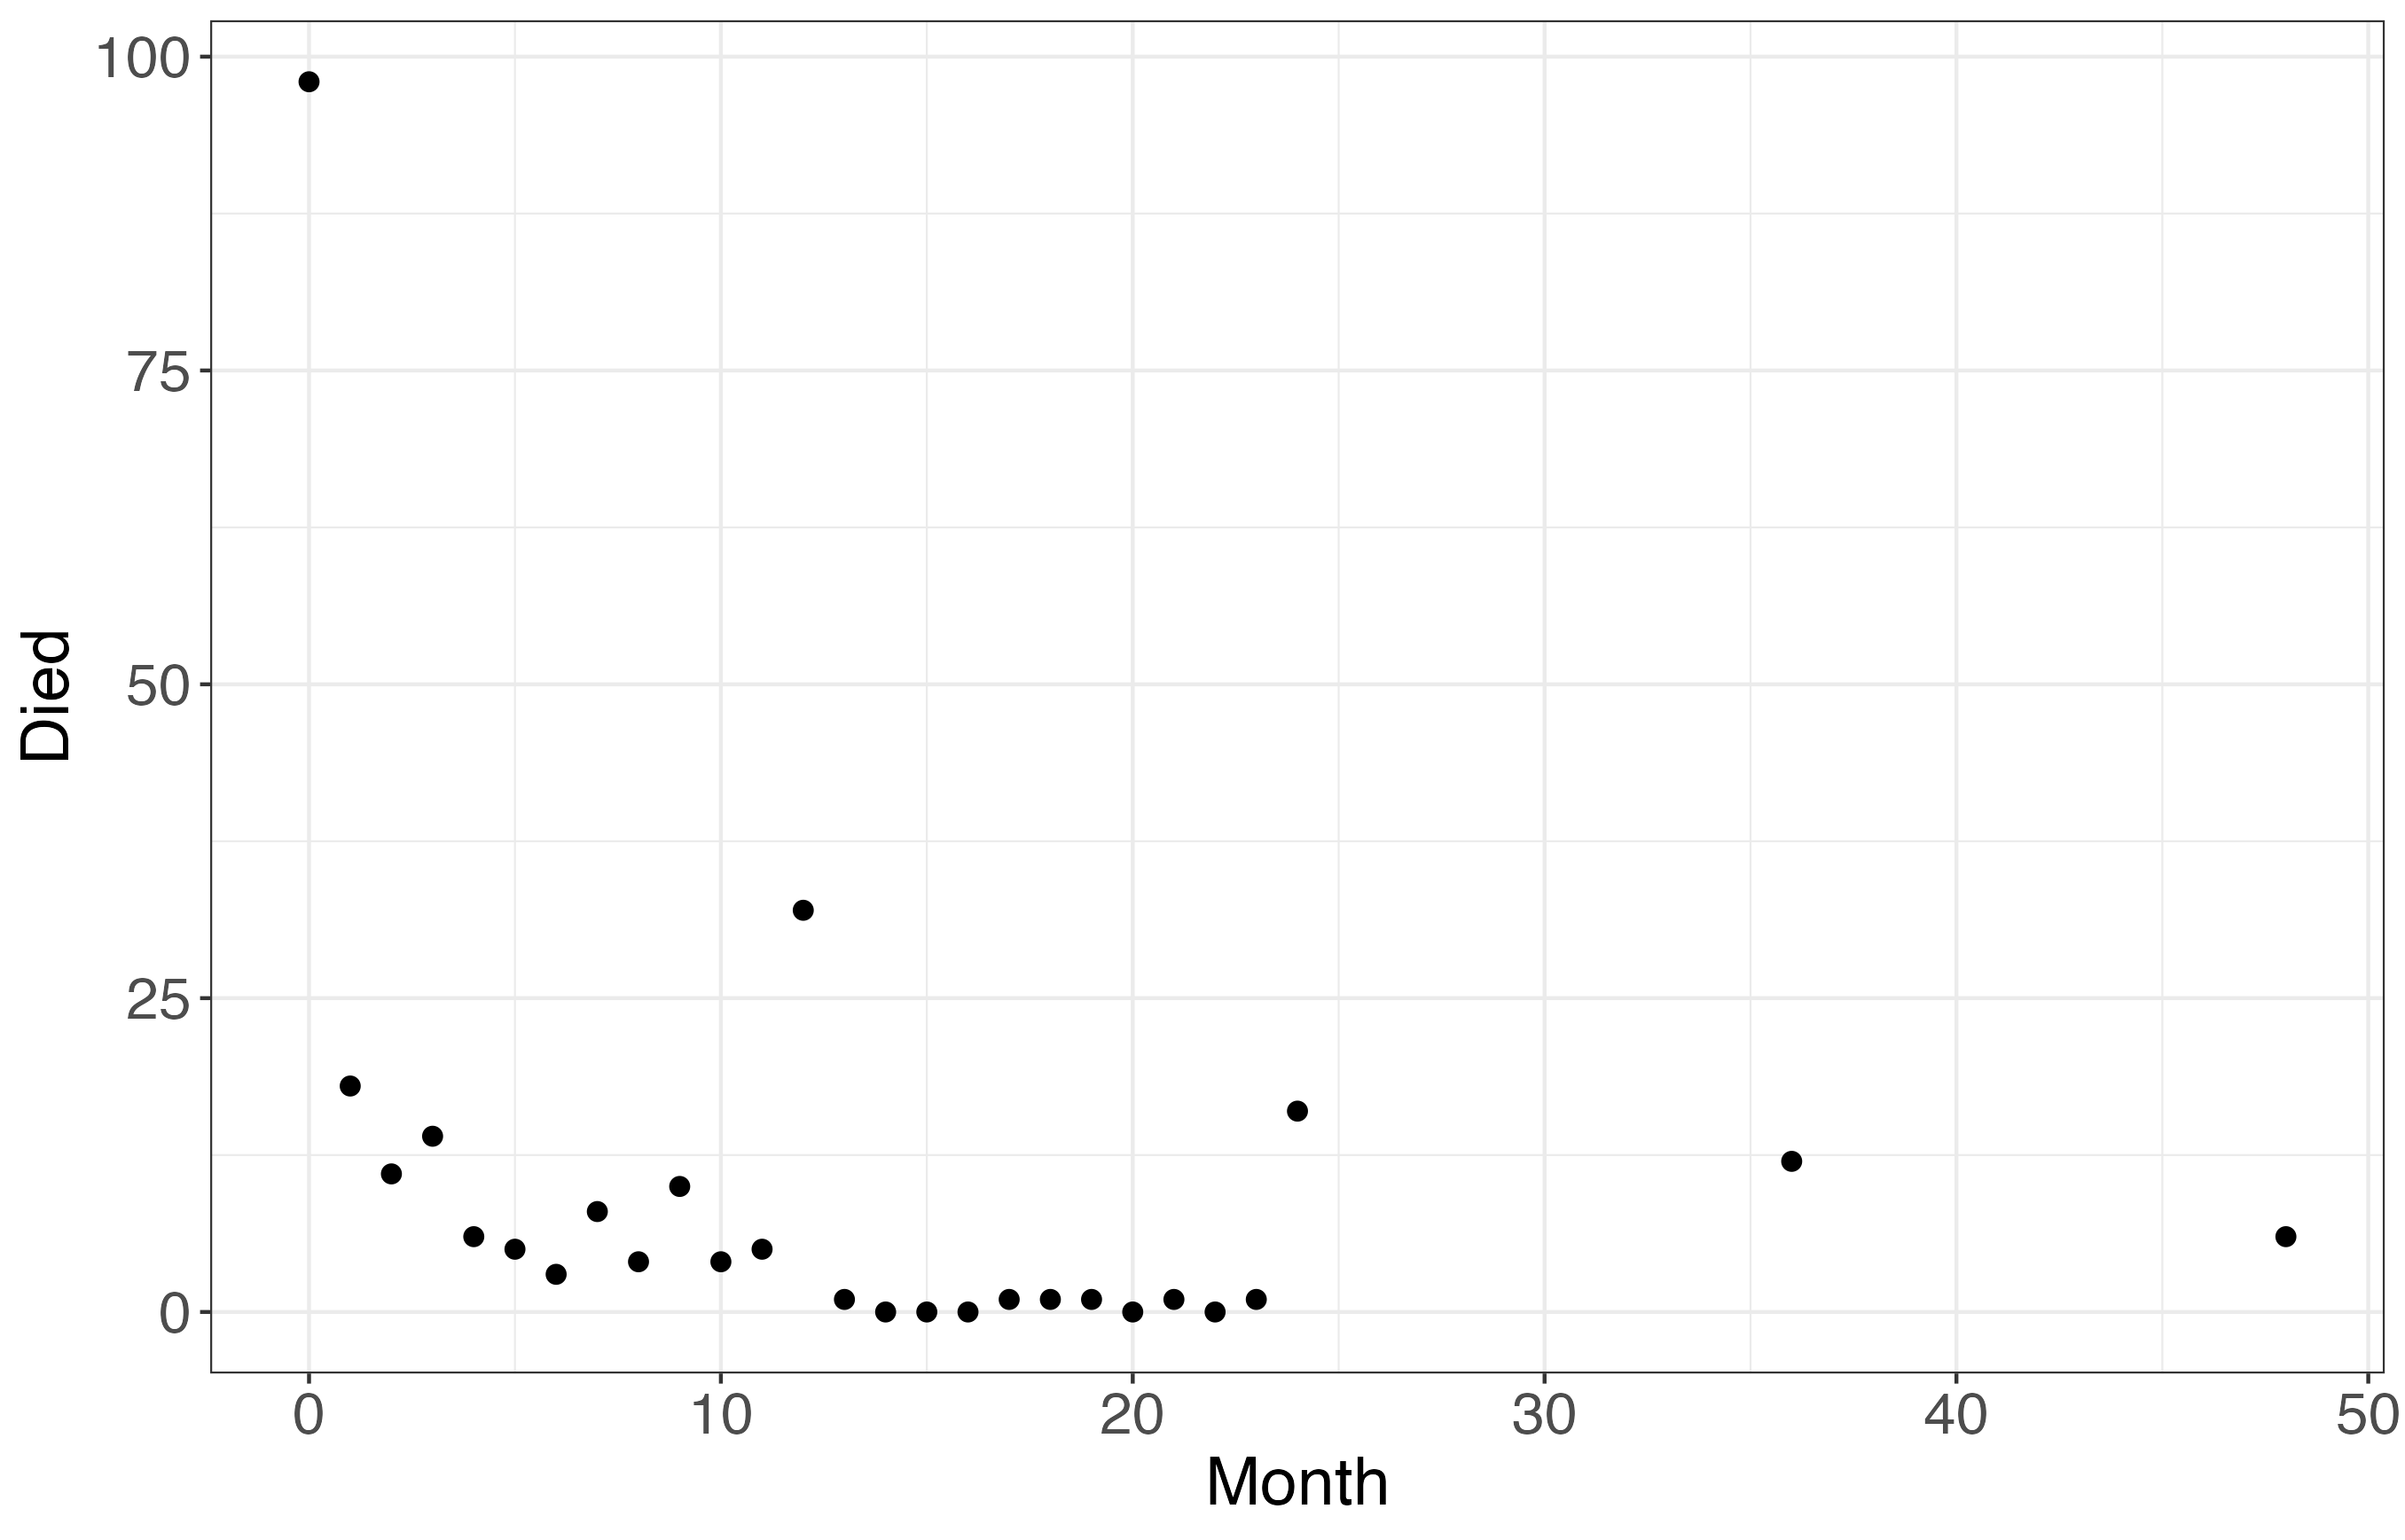
\includegraphics[scale=0.3]{u5mr.png}
\end{frame}

\begin{frame}
\begin{figure}
	\centering 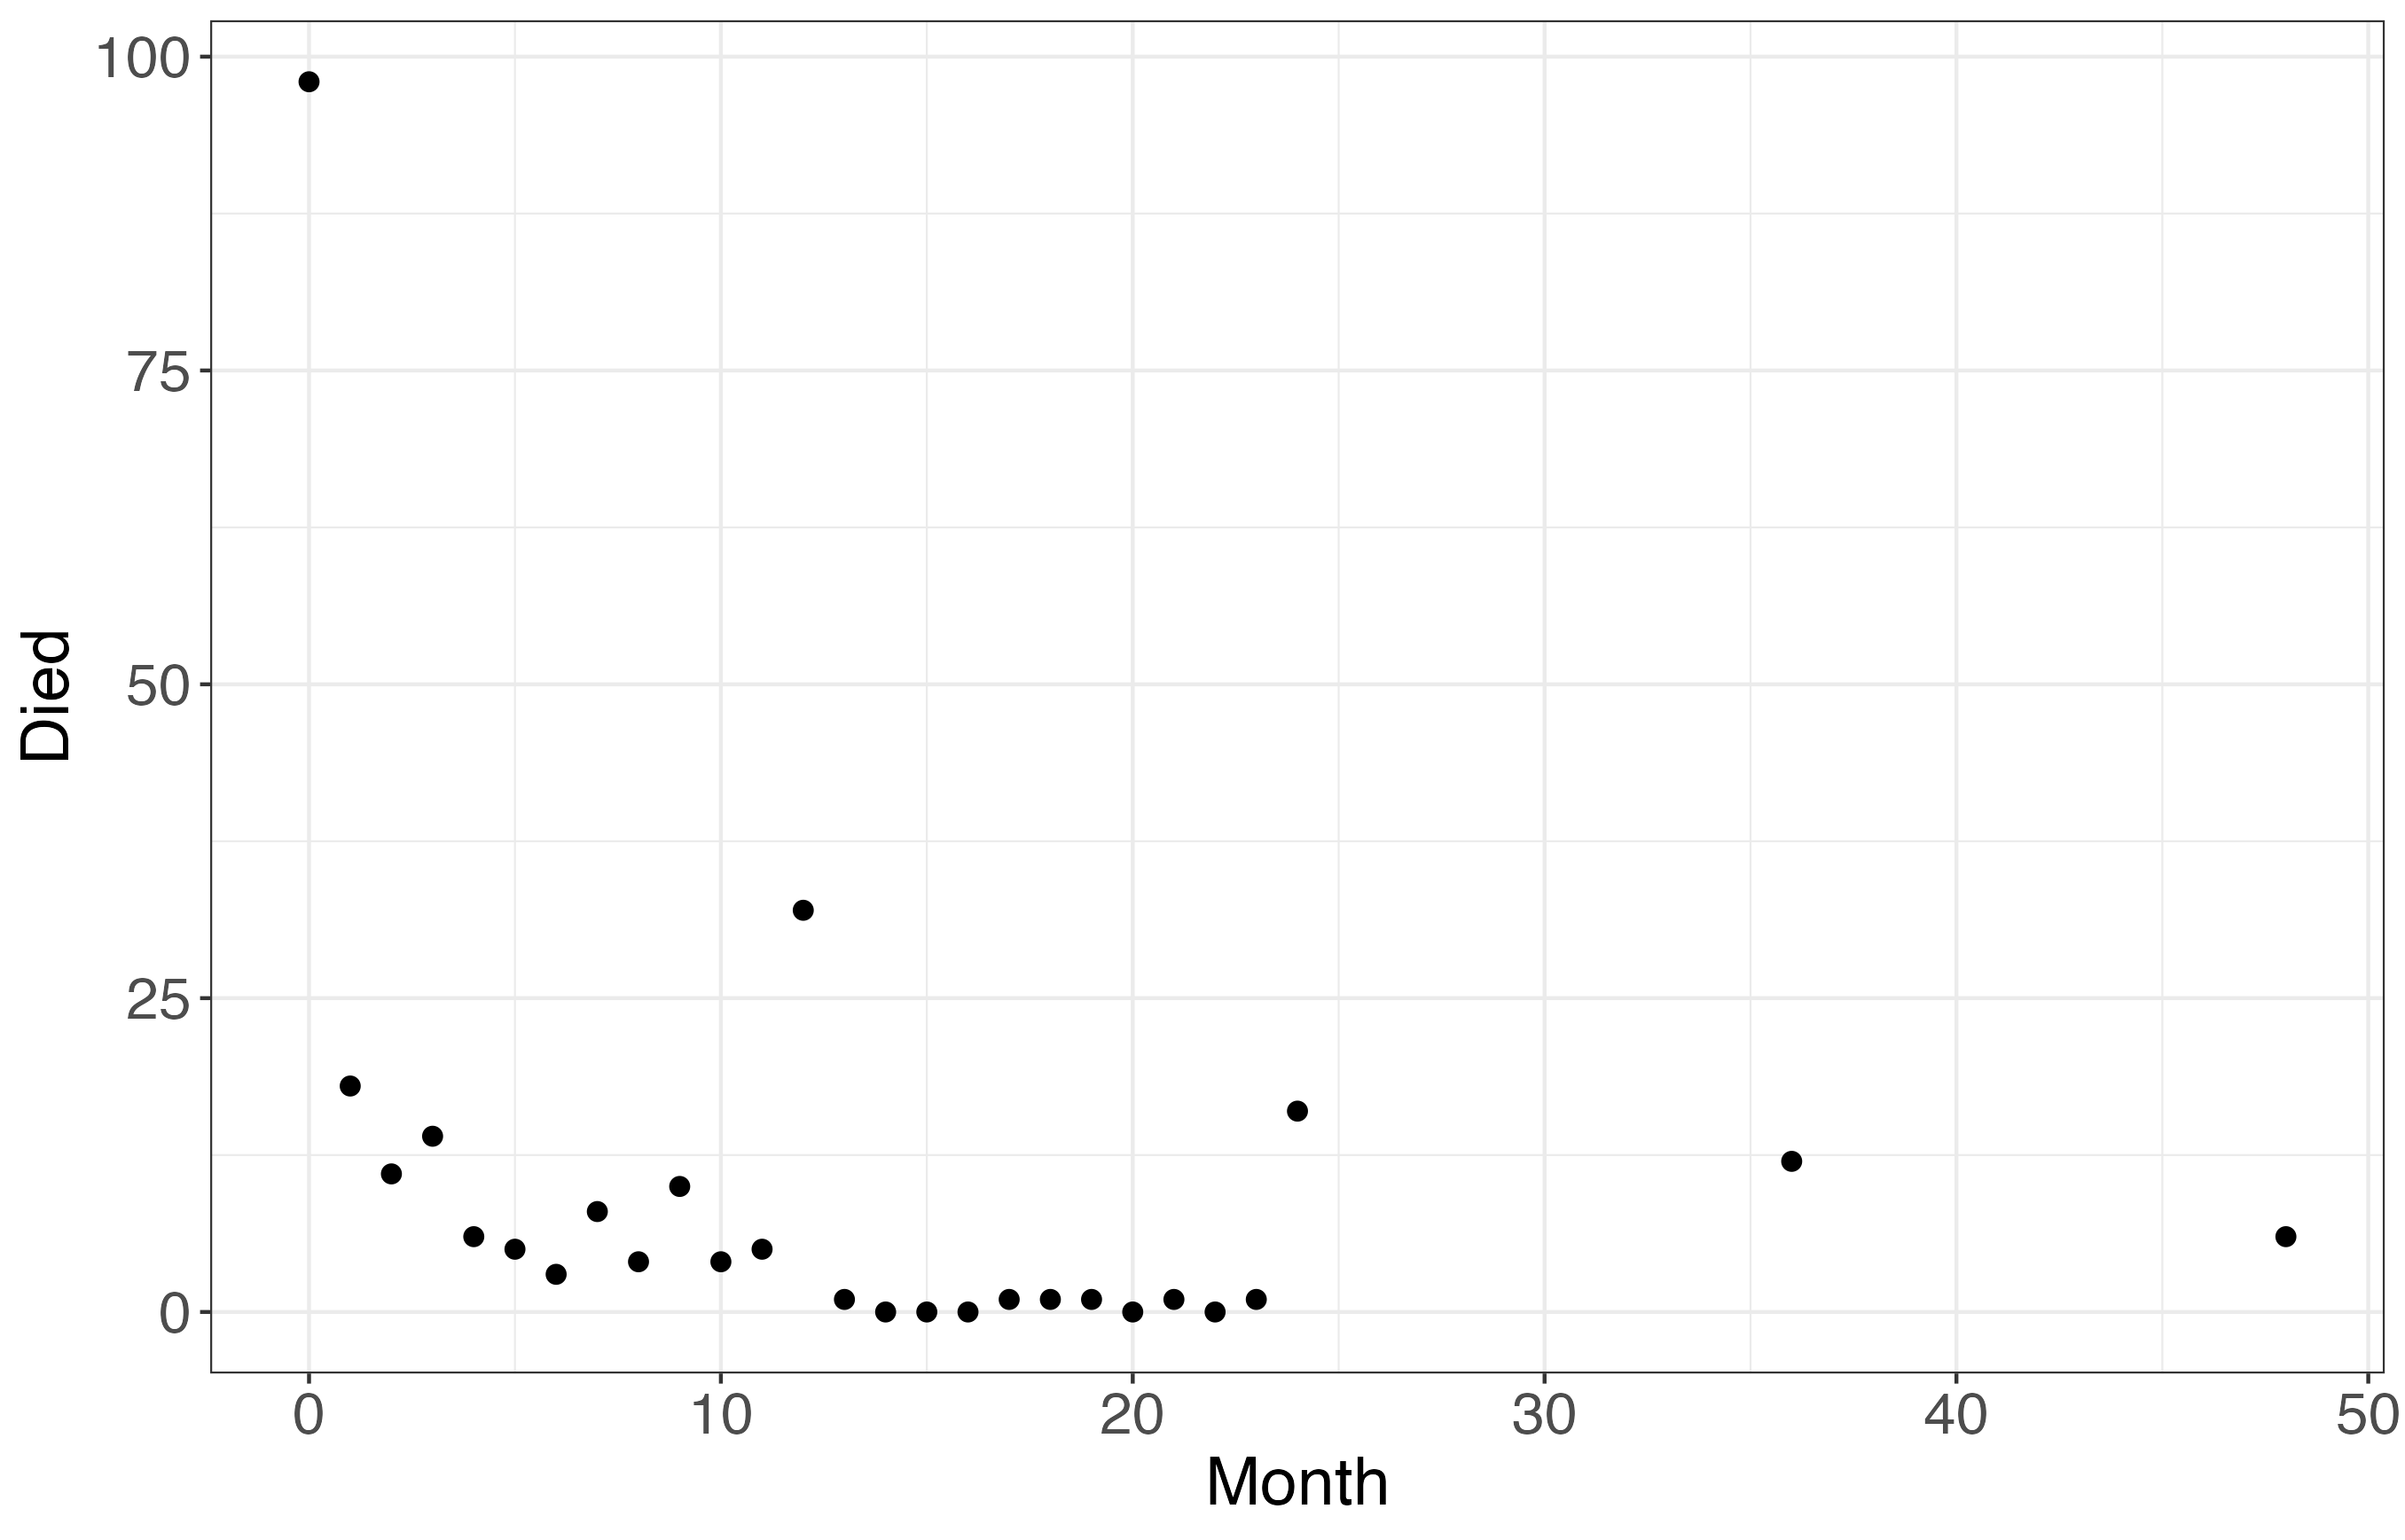
\includegraphics[scale=0.3]{u5mr.png}
\end{figure}
	
\vspace{0.3cm}

\begin{itemize}
	\item Argue why we should consider age at death to be a continuous variable.
	\item Argue why we should consider age at death to be a discrete variable.
	\item Do you notice anything strange about the plot? Does this affect whether or not we should consider age at death to be continuous or discrete?
\end{itemize}

\end{frame}

\begin{frame}

Argue why we should consider age at death to be a continuous variable.
	
	\vspace{0.3cm}
	
	\begin{itemize}
		\item[] \textcolor{blue}{Age is inherently continuous. We could, in theory, have ages recorded with an infinite number of decimal points.}
	\end{itemize}
	
		
	
	\vspace{0.3cm}
	
	Argue why we should consider age at death to be a discrete variable.
	
	\vspace{0.3cm}
	
	\begin{itemize}
		\item[] 	\textcolor{blue}{Age is collected discretely in the survey. According to the survey, children could not be 2.5 years old, for example. }
	\end{itemize}

	

\end{frame}

\begin{frame}

	
Do you notice anything strange about the plot? Does this affect whether or not we should consider age at death to be continuous or discrete?
	
	\vspace{0.3cm}
	
\begin{itemize}
	\item[] \small \textcolor{blue}{Death counts seem to be higher at exact years than for the months in between 1-2 years. For 24 months, 3 years, and 4 years, this is likely due to grouping. If a child died between ages 2.5 - 3.5, they would be recorded as having died at 3 years, so this count would be inherently higher since it spans a longer time period than simply 1 month. However, what about 12 months?} 
	
	\vspace{0.3cm}
	
	\item[] \small \textcolor{blue}{This phenomenon is known as ``age-heaping", and often occurs in surveys where parents do not know the exact age their child was when they died, or when surveyers themselves record dates inexactly. This is essentially a rounding error, where many deaths are recorded at 1 year even though they may have occurred at any time between 0 and 2 years. }
\end{itemize}	
	
	

	\vspace{0.3cm}

Considering age to be continuous \textit{or} discrete in this example are both justifiable conclusions! In general, we'll consider age to be continuous in this class, but in specific scenarios it may make more sense to consider age in discrete, ordinal groups.

\end{frame}

\subsection{Descriptive Statistics}

\begin{frame}{Descriptive Statistics}
Why do we need descriptive statistics?

\vspace{0.3cm}

\begin{itemize}
	\item Making sense of large amounts of data
	\item Checking data quality
	\begin{itemize}
		\item Values outside reasonable range (e.g., height = 9')
		\item Implausible combinations of variables (e.g., positive test for cervical cancer for a person without a cervix)
	\end{itemize}
	\item Observe distribution of variables in dataset
	\begin{itemize}
		\item Measures of center and spread
	\end{itemize}
	\item Start to understand direction and strength of association
	\begin{itemize}
		\item Descriptive statistics and inferential statistics should contribute to the same story
	\end{itemize}
\end{itemize}

\end{frame}

\begin{frame}{Descriptive Statistics}
Appropriate descriptive statistics will vary depending on what how many variables you want to describe at once, and whether or not you want numerical or graphical summaries.

\vspace{0.3cm}

Outline:
\begin{itemize}
	\item Univariate
	\begin{itemize}
		\item Numerical (categorical variables)
		\item Numerical (quantitative variables)
	\end{itemize}
	\item Stratified/Bivariate
	\begin{itemize}
		\item Numerical summaries, broken down by group
		\item Graphical
	\end{itemize}
\end{itemize}
\end{frame}

\subsubsection{Univariate}

\begin{frame}{Univariate Descriptive Statistics: Categorical}
\textcolor{blue}{Example:} In our GHI dataset, we have information on the urban population of each country (the proportion of people living in urban areas vs. rural areas). We consider the following three categories for a country in a given year:

\vspace{0.3cm}

\begin{itemize}
	\item Highly urban: 70\% or more
	\item Somewhat urban: 40\% to 69\%
	\item Not very urban: 0\% to 39\%
\end{itemize}

\vspace{0.3cm}

Suppose we are interested in knowing how many countries fall into each group in 2014. How would we summarize this data?

\end{frame}

\begin{frame}{Univariate Descriptive Statistics: Categorical}

We could begin by counting up the number of countries that fall in each category:

\vspace{0.3cm}

\begin{table}
	\centering
	\begin{tabular}{l|r}
		\textbf{Urbanicity} & \textbf{Number of Countries} \\
		\hline
		High & 64\\
		\hline
		Medium & 78\\
		\hline
		Low & 50\\
		\hline 
		NA & 1
	\end{tabular}
\end{table}


\vspace{0.3cm}

Note that one country (Eritrea) in our dataframe does not have any urbanicity information in 2014!

\end{frame}

\begin{frame}{Univariate Descriptive Statistics: Categorical}
We can also report the proportion of countries that fall in each group:

\vspace{0.3cm}

\begin{table}
	\centering
	\begin{tabular}{l|r}
		\textbf{Urbanicity }& \textbf{Proportion of Countries (No.)} \\
		\hline
		High & 33.3\% (64)\\
		\hline
		Medium & 40.6\% (78)\\
		\hline
		Low & 26.0\% (50)\\
		\hline 
		NA & 0.5\% (1)
	\end{tabular}
\end{table}

\end{frame}

\begin{frame}{Univariate Descriptive Statistics: Categorical}
Summary should include:

\vspace{0.3cm}

\begin{itemize}
	\item Number and percent in each group
	\item If binary, only need to summarize one group
	\begin{itemize}
		\item The other can be inferred (for example, if 30\% of the population have a genetic variant, 100 - 30 = 70\% do not.)
	\end{itemize}
	\item Also good to summarize missing data
	\begin{itemize}
		\item e.g., \# and proportion of missing values
	\end{itemize}
\end{itemize}	
\end{frame}

\begin{frame}{Univariate Descriptive Statistics: Quantitative}

\textcolor{blue}{Example:} Rather than considering three groups for urbanicity, we could consider urban proportion as a quantitative measure ranging from 0\% to 100\%. The dataset for the year 2014 looks like \dots

\vspace{0.3cm}

\begin{table}
	\centering
	\begin{tabular}{l|r}
		\textbf{Country} & \textbf{Urban \%} \\
		\hline
		Afghanistan & 24.587\\
		\hline
		Angola & 62.731\\
		\hline
		Albania & 56.423 \\
		\hline 
		\vdots & \vdots \\
		\hline
		South Africa & 64.312 \\
		\hline 
		Zambia & 41.382 \\
		Zimbabwe & 32.504
	\end{tabular}
\end{table}

\vspace{0.3cm}

What information may be useful to know?

\end{frame}

\begin{frame}{Univariate Descriptive Statistics: Quantitative}

How many countries are in our dataset?

\begin{itemize}
	\item[] \textcolor{blue}{There are 193 countries in our dataset.}
\end{itemize}

Do any countries have missing values for percent urban?

\begin{itemize}
	\item[] \textcolor{blue}{1 country has missing information for percent urban in 2014 (Eritrea).}
\end{itemize}

Measures of center?

\begin{itemize}
	\item[] \textcolor{blue}{Mean percent urban is 57.8\%}
	\item[] \textcolor{blue}{Median percent urban is 57.6\%} 
\end{itemize}

Measures of spread?

\begin{itemize}
	\item[] \textcolor{blue}{Sample standard deviation is 23.1\%}
	\item[] \textcolor{blue}{Interquartile range (IQR) is (39.5\%, 76.9\%) (Q1, Q3)}
	\item[] \textcolor{blue}{Range is (11.8\%, 100\%) (Burundi has the lowest percent urban, Kuwait, Monaco, Nauru, and Singapore are tied for the highest percent urban)}
\end{itemize}


\end{frame}
	
\begin{frame}{Univariate Descriptive Statistics: Quantitative}
Summary should include (some of):

\vspace{0.3cm}

\begin{itemize}
	\item Sample size / number of observations
	\item Number of missing observations
	\item Measures of center:
	\begin{itemize}
		\item Sample mean
		\item Sample median
	\end{itemize}
	\item Measures of spread:
	\begin{itemize}
		\item Sample standard deviation
		\item Interquartile range (IQR): (Q1, Q3) or (Q3 - Q1)
		\item Range: (Min, Max) or (Max - Min)
	\end{itemize}
\end{itemize}

\end{frame}

\begin{frame}{Univariate Descriptive Statistics: Graphical}
For categorical variables, we can make barplots:

\vspace{0.3cm}

\centering 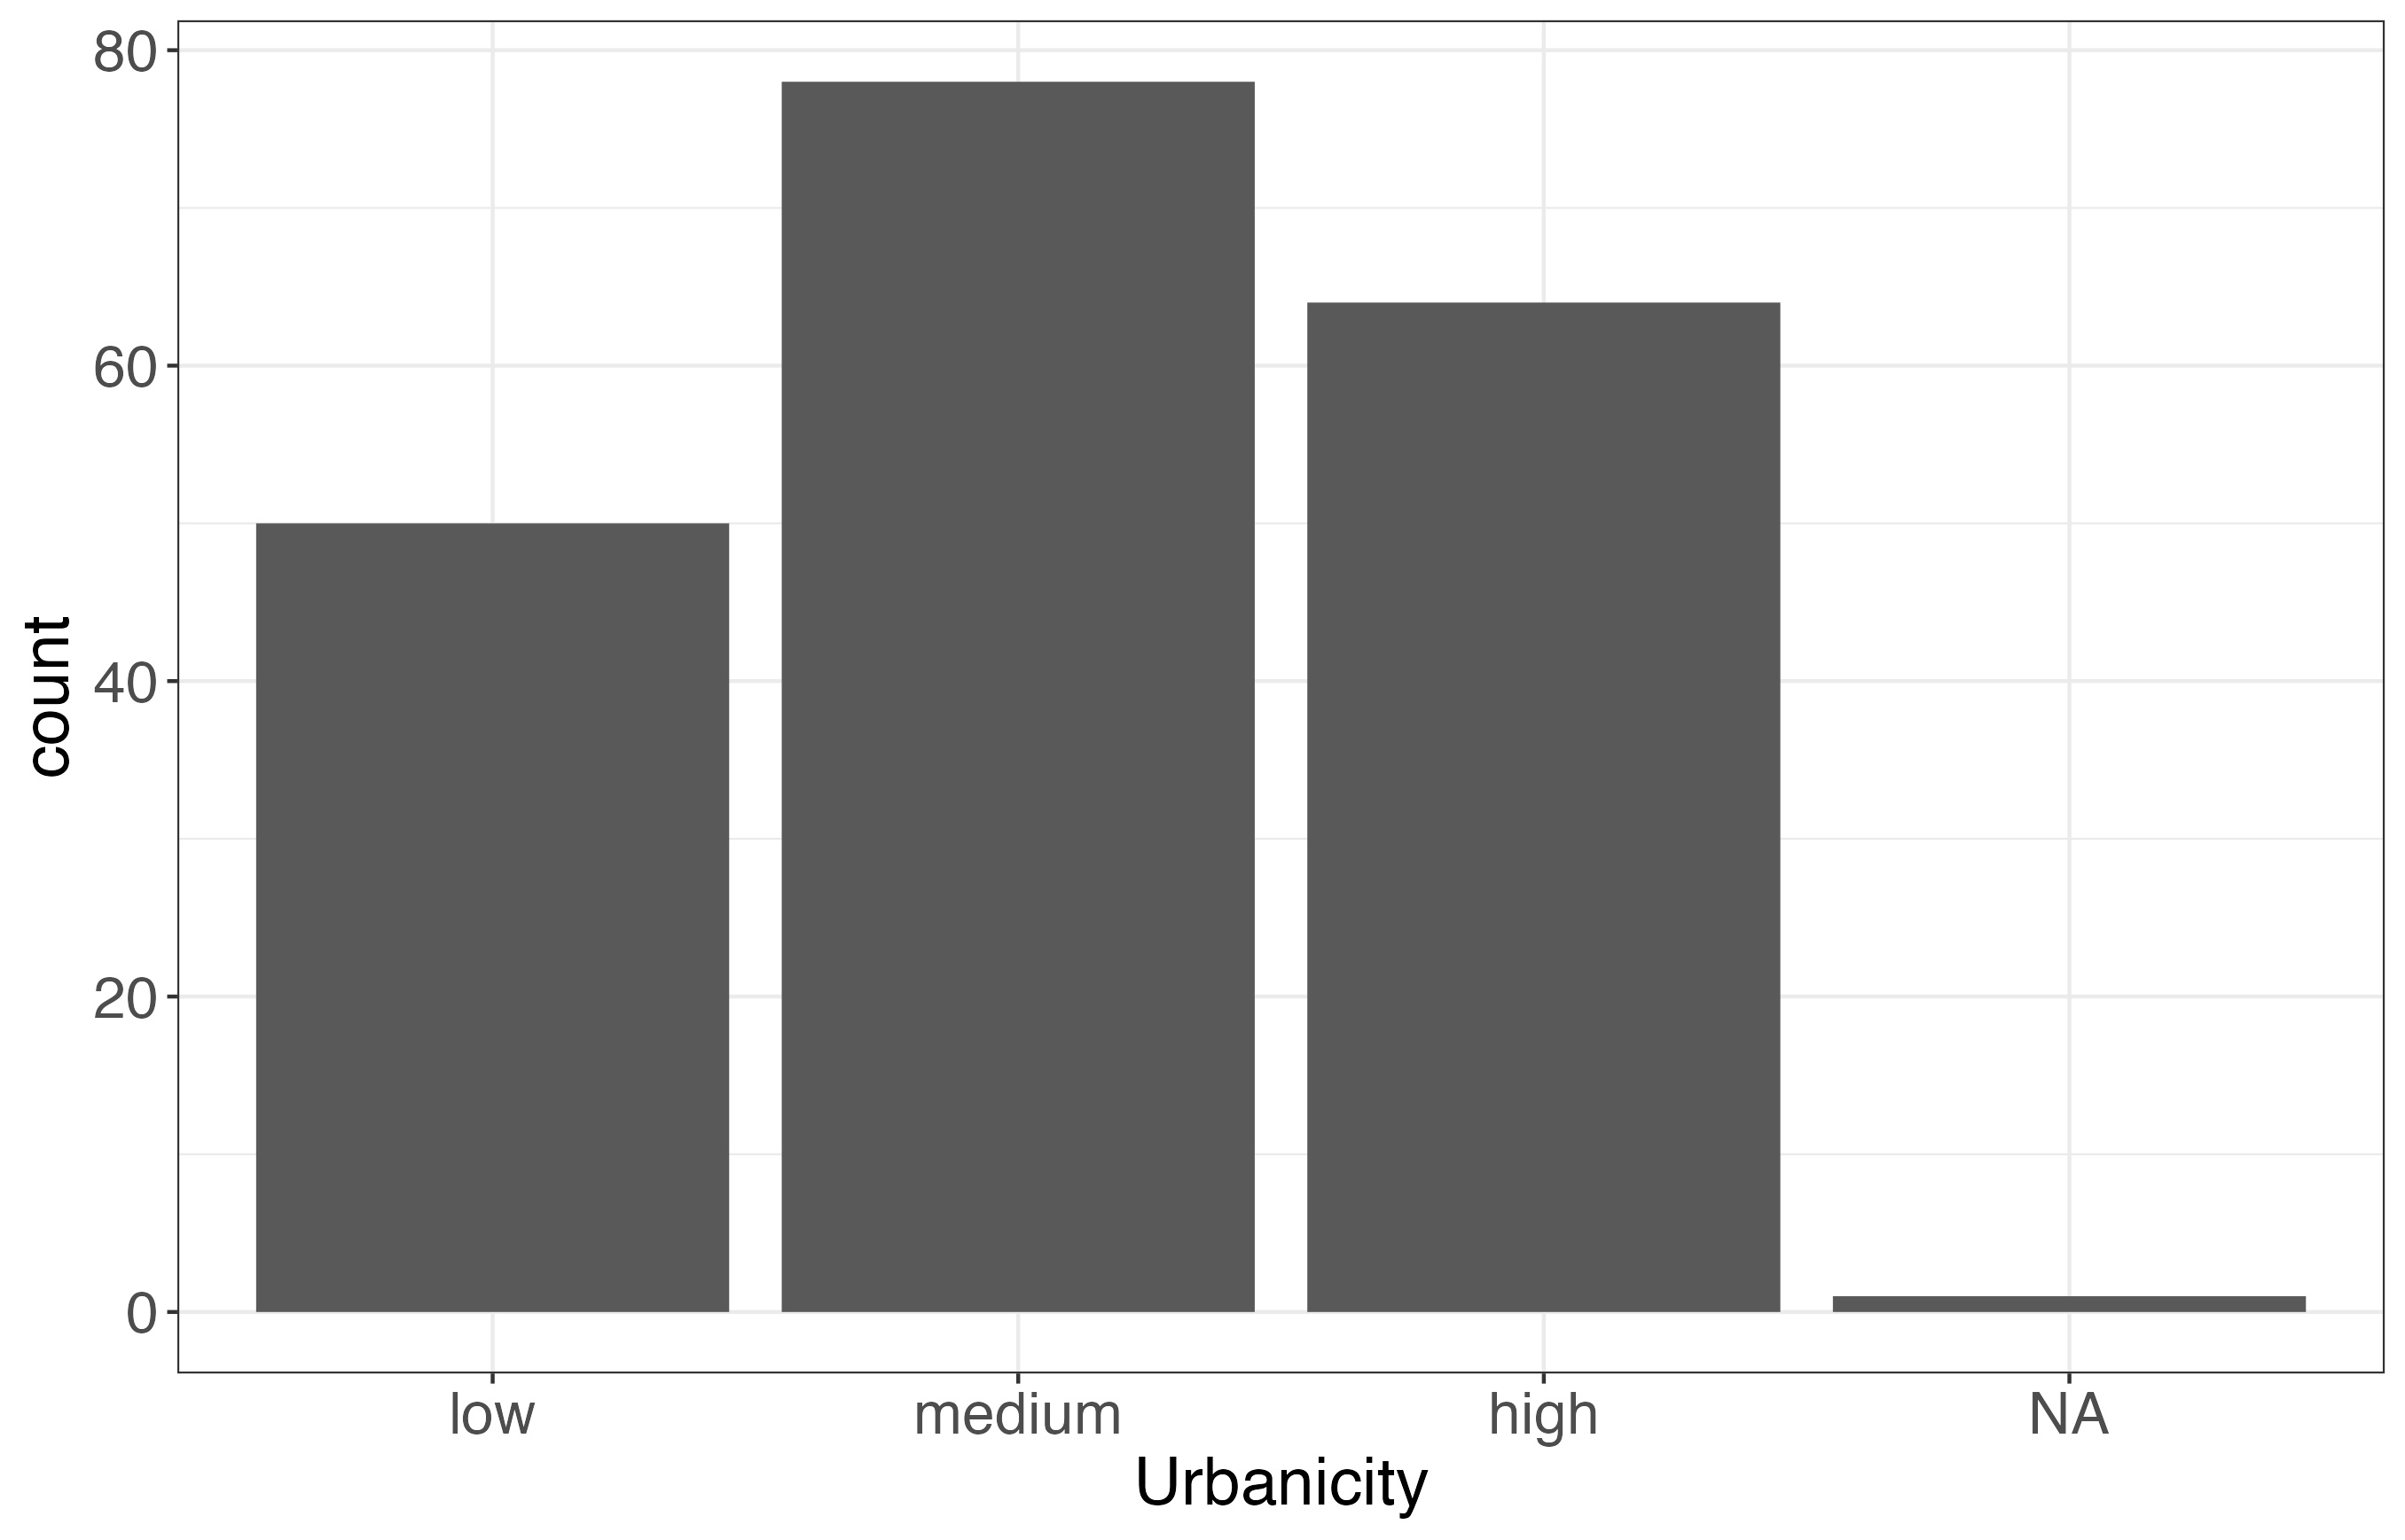
\includegraphics[scale=0.4]{urban_barplot.png}

\end{frame}

\begin{frame}{Univariate Descriptive Statistics: Graphical}
For quantitative variables, we can make histograms and boxplots. Histograms are useful for describing the shape of the distribution of a variable, and boxplots are useful for seeing central tendancy (and sometimes outliers):

\vspace{0.4cm}

\begin{figure}
	\centering
	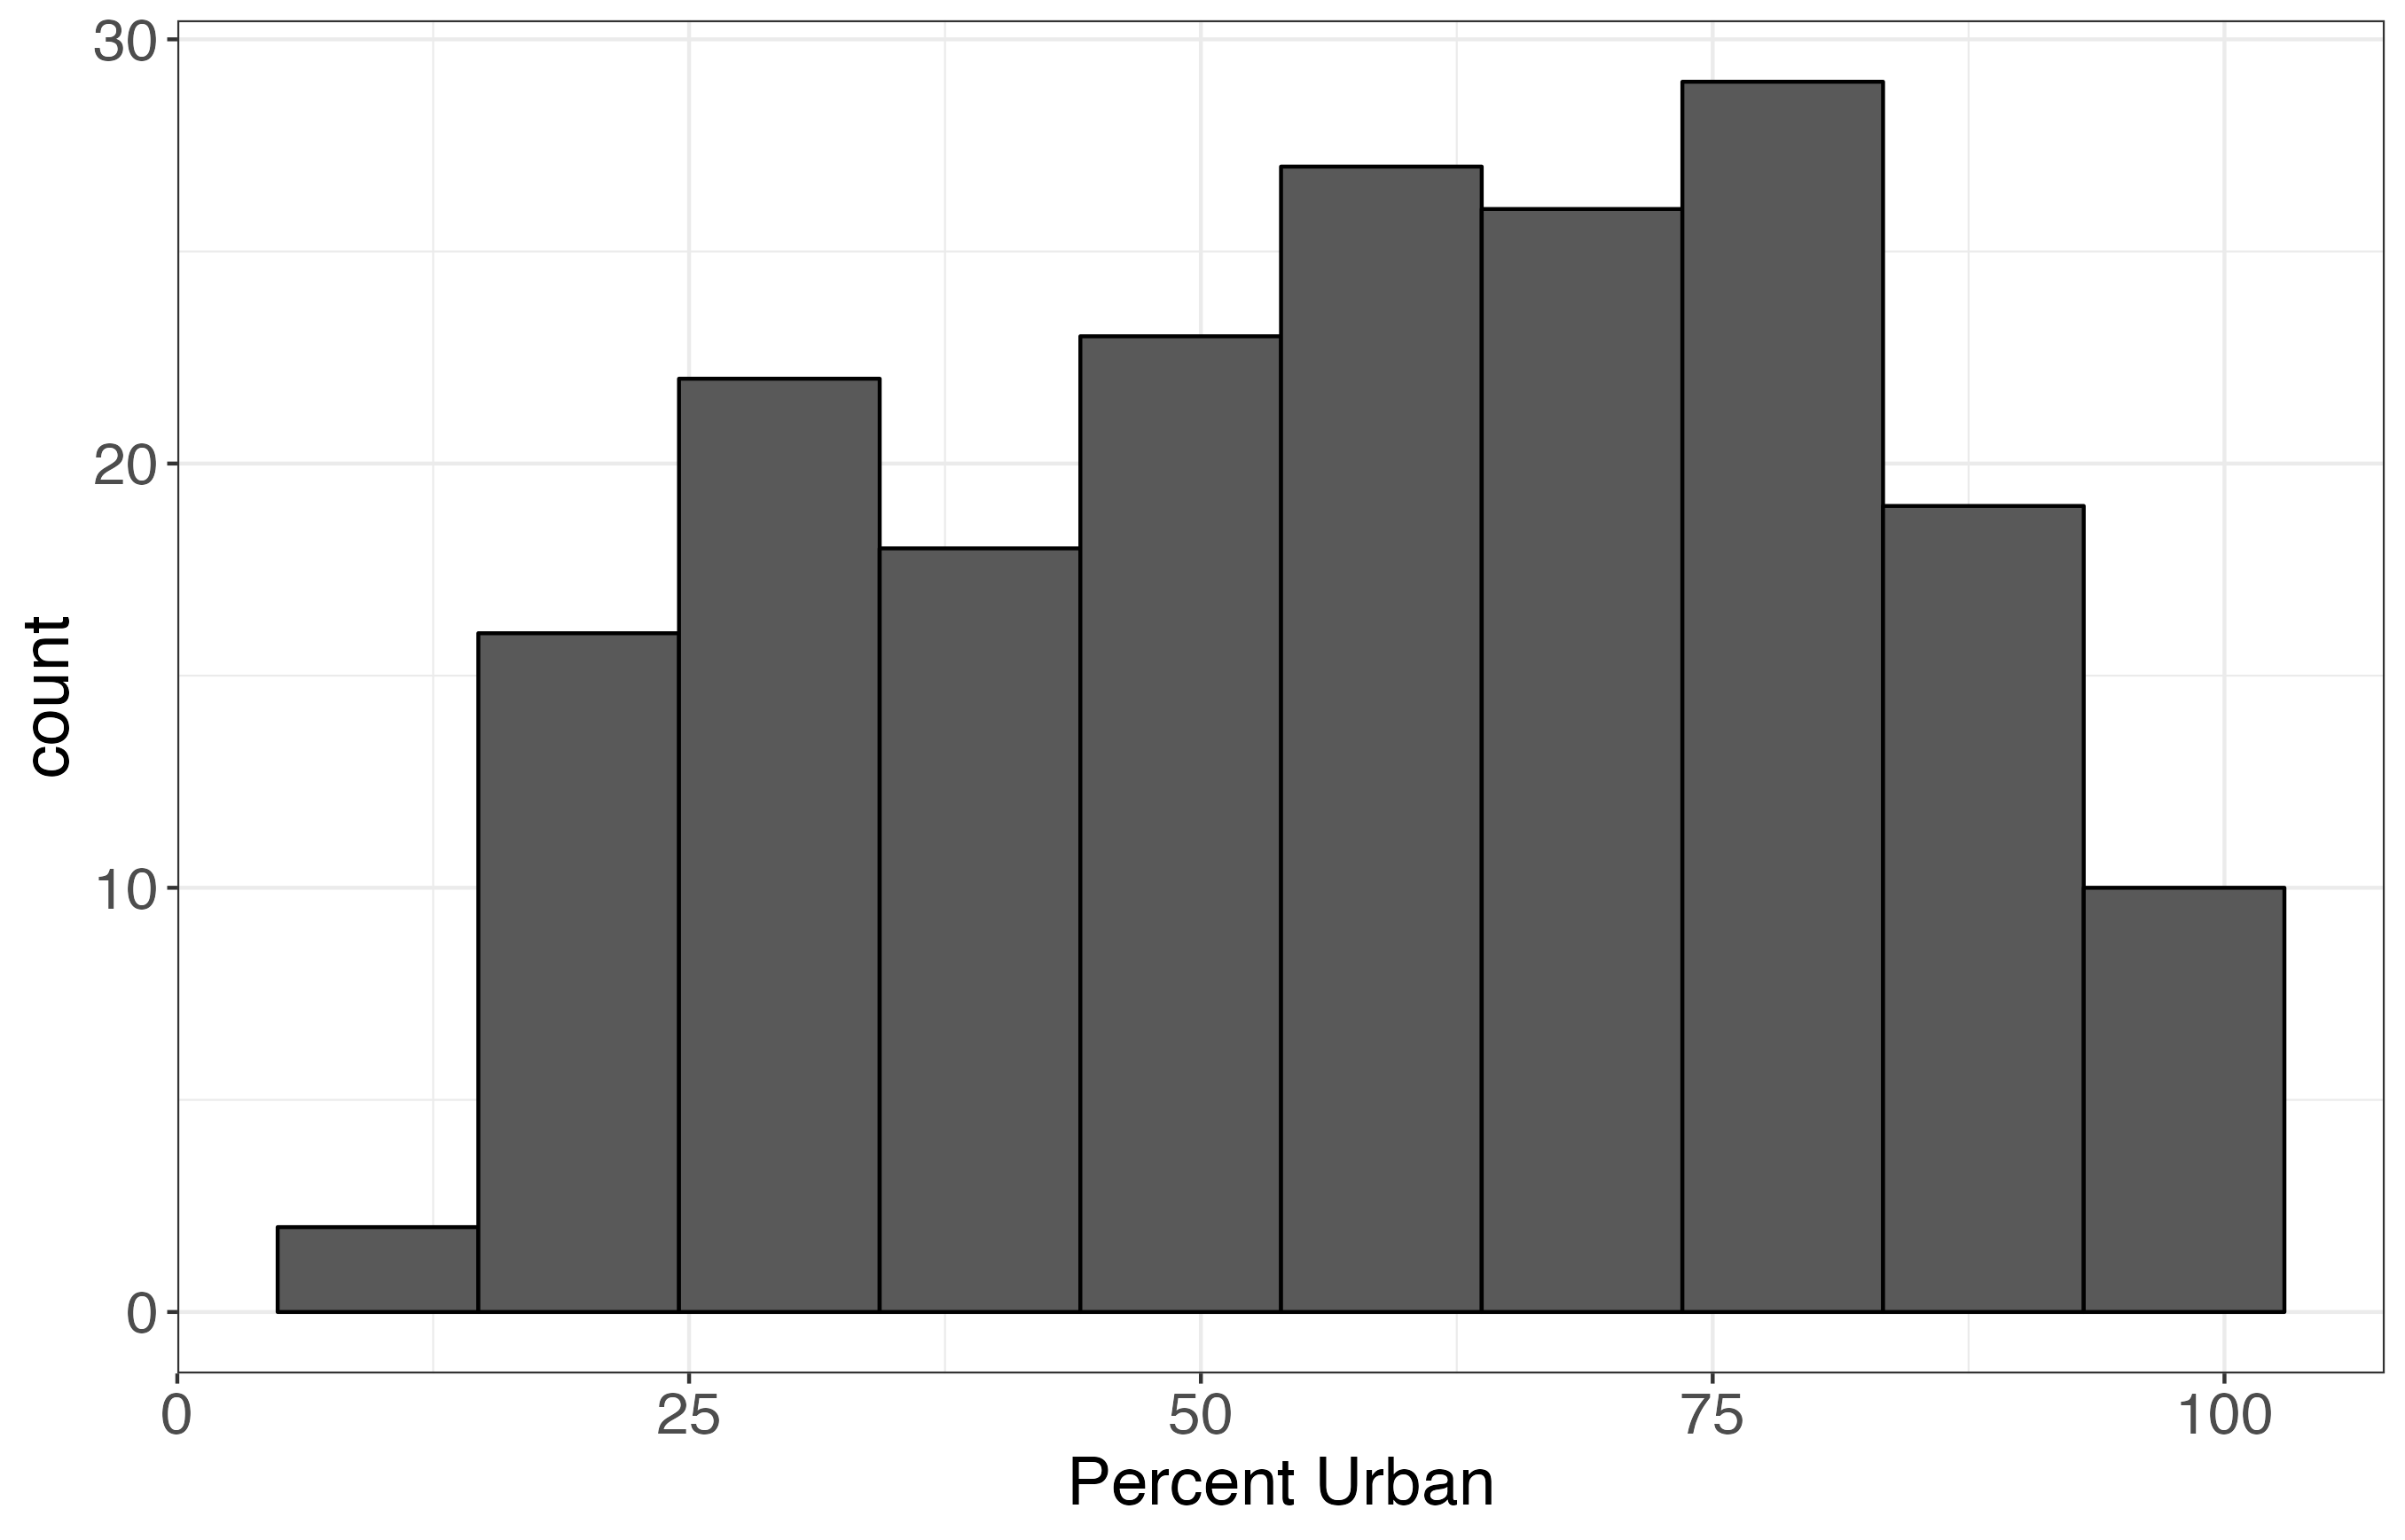
\includegraphics[scale=0.2]{urban_hist.png}
	\hspace{0.2cm}
	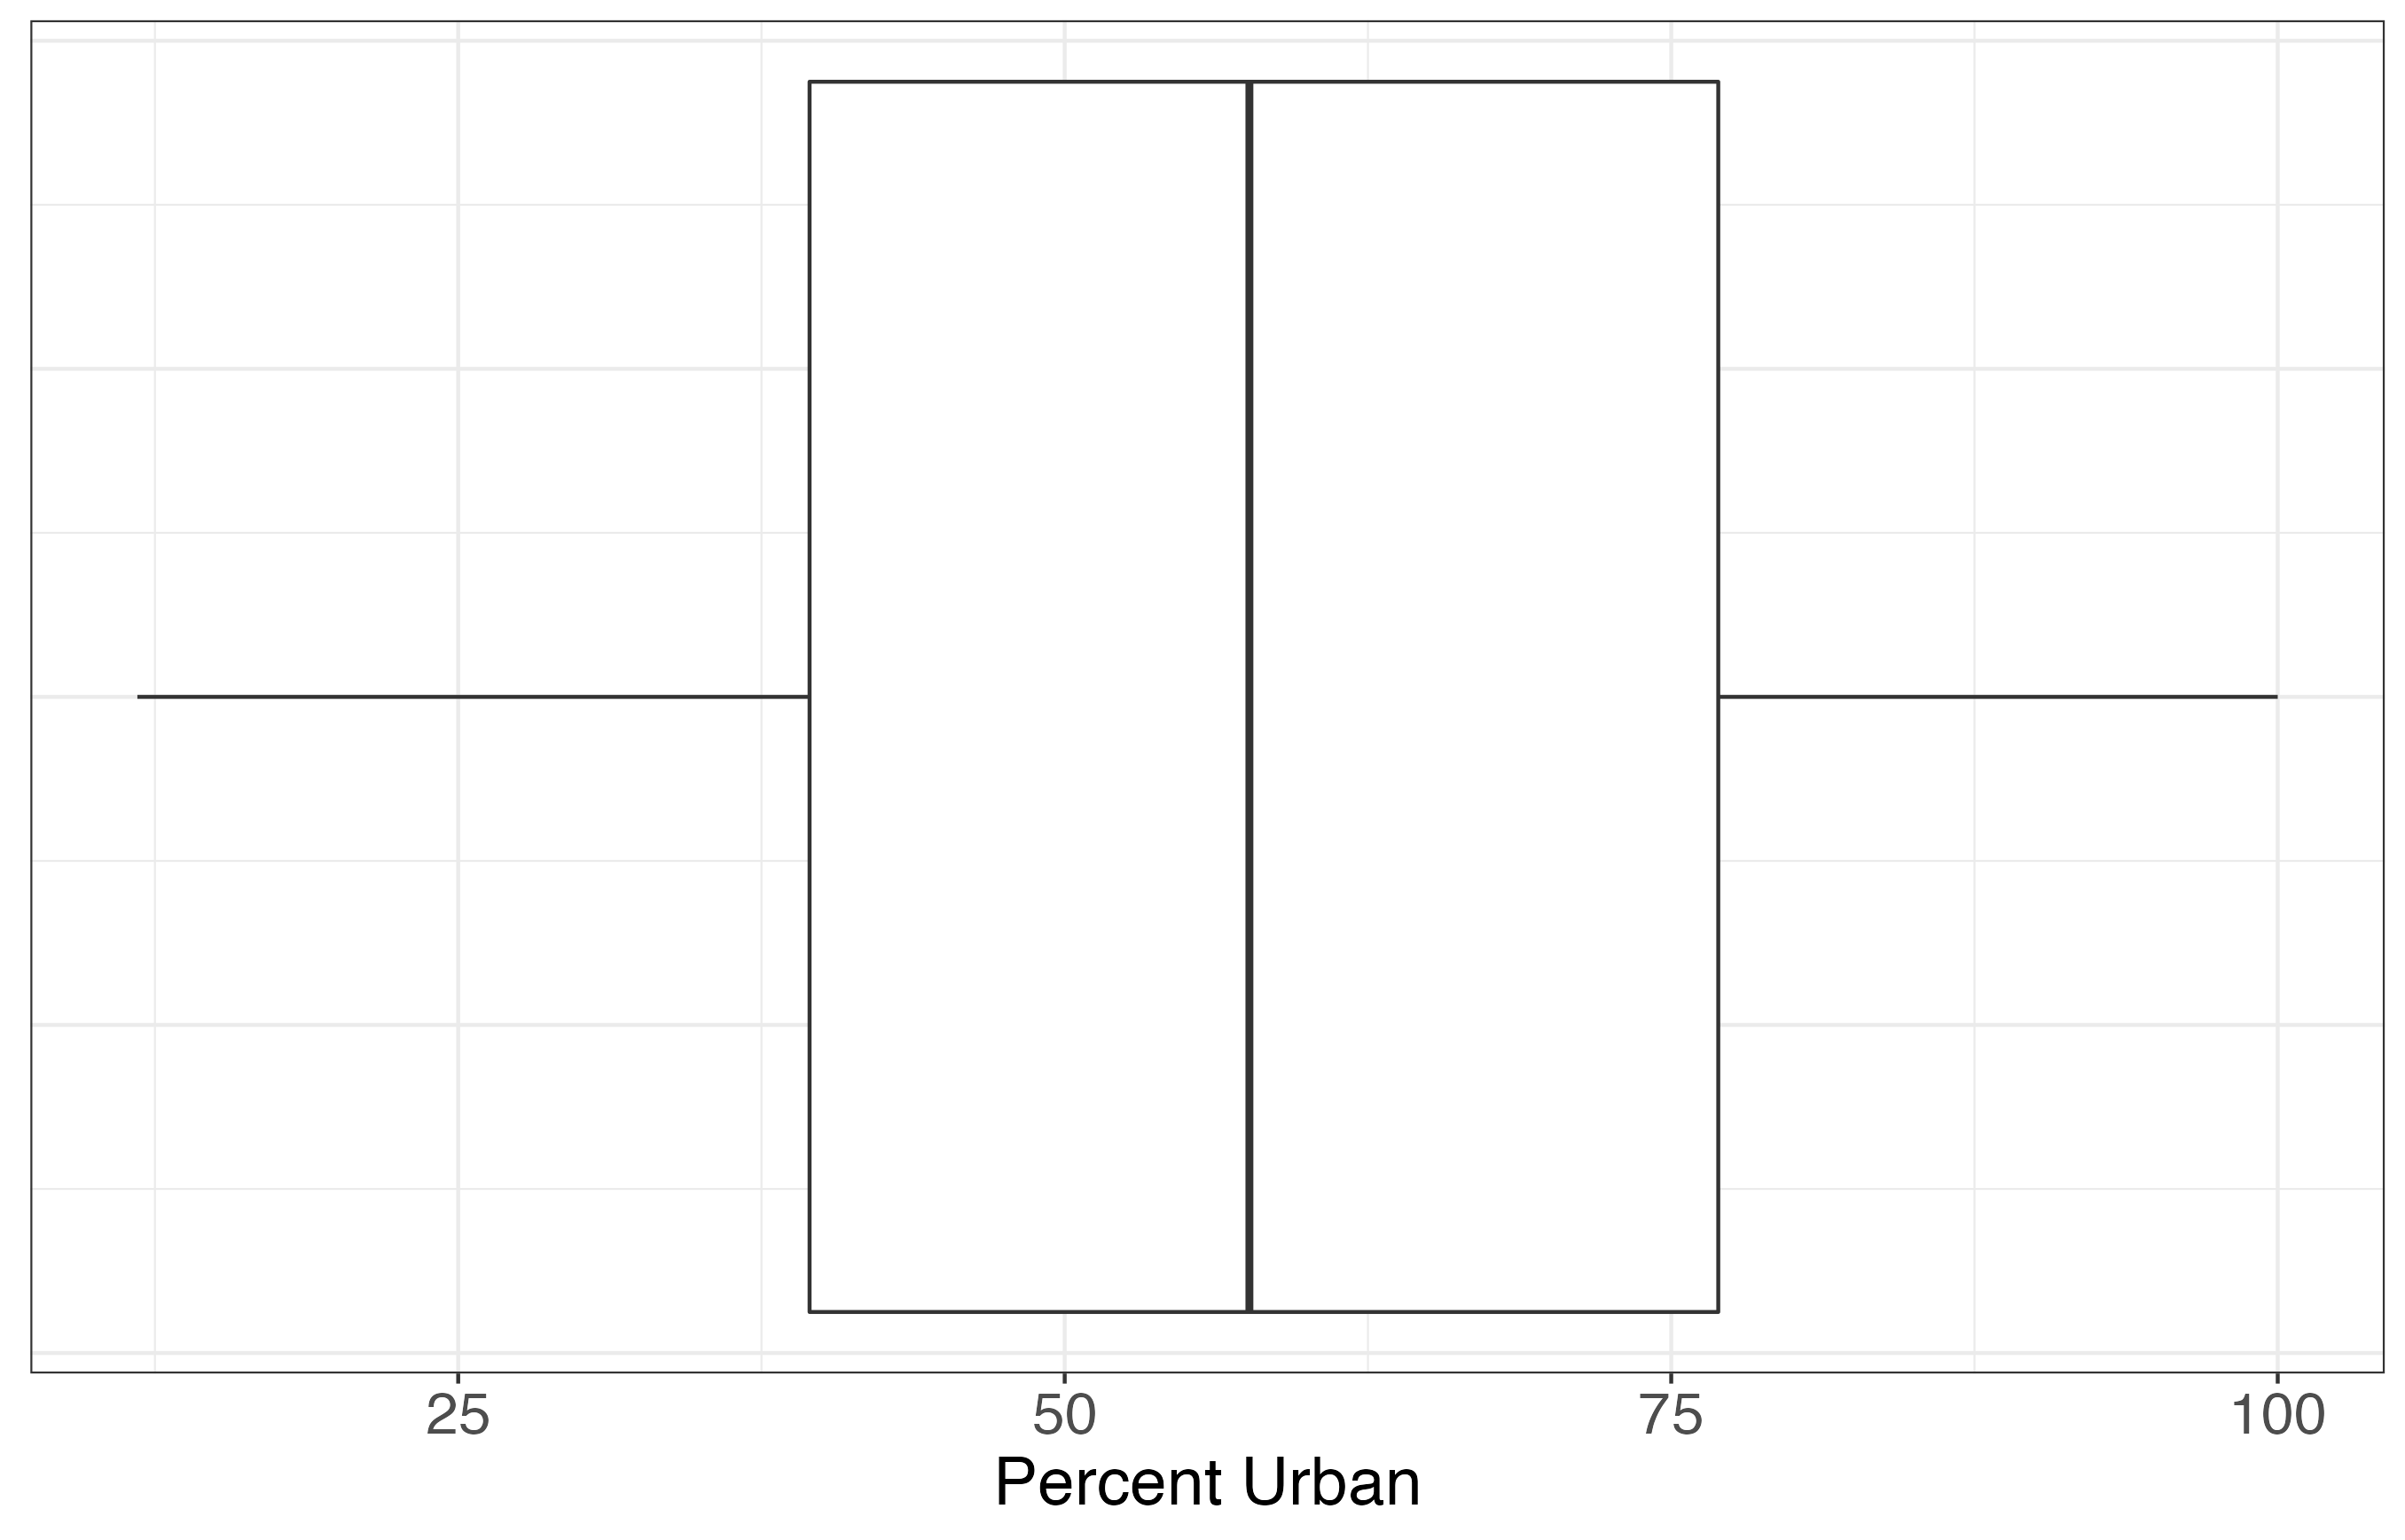
\includegraphics[scale=0.2]{urban_box.png}
\end{figure}

\end{frame}

\subsubsection{Stratified/Bivariate}

\begin{frame}{Stratified Descriptive Statistics: Graphical}
Sometimes we're interested in the distribution of a variable within certain subgroups, rather than across all the data:

\vspace{0.3cm}

\begin{itemize}
	\item e.g., how does the distribution of percent urban differ between years in our GHI dataset?
\end{itemize}

\vspace{0.3cm}

Stratified descriptive statistics can help us:

\vspace{0.3cm}

\begin{itemize}
	\item Understand the role of the stratification variable
	\item Begin to demonstrate the association between the two variables
\end{itemize}

\end{frame}

\begin{frame}{Stratified Descriptive Statistics: Graphical}

How does the distribution of percent urban differ between years in our GHI dataset? We can make histograms for the years 2000, 2005, 2010, and 2015, and 2020:

\vspace{0.3cm}

\centering 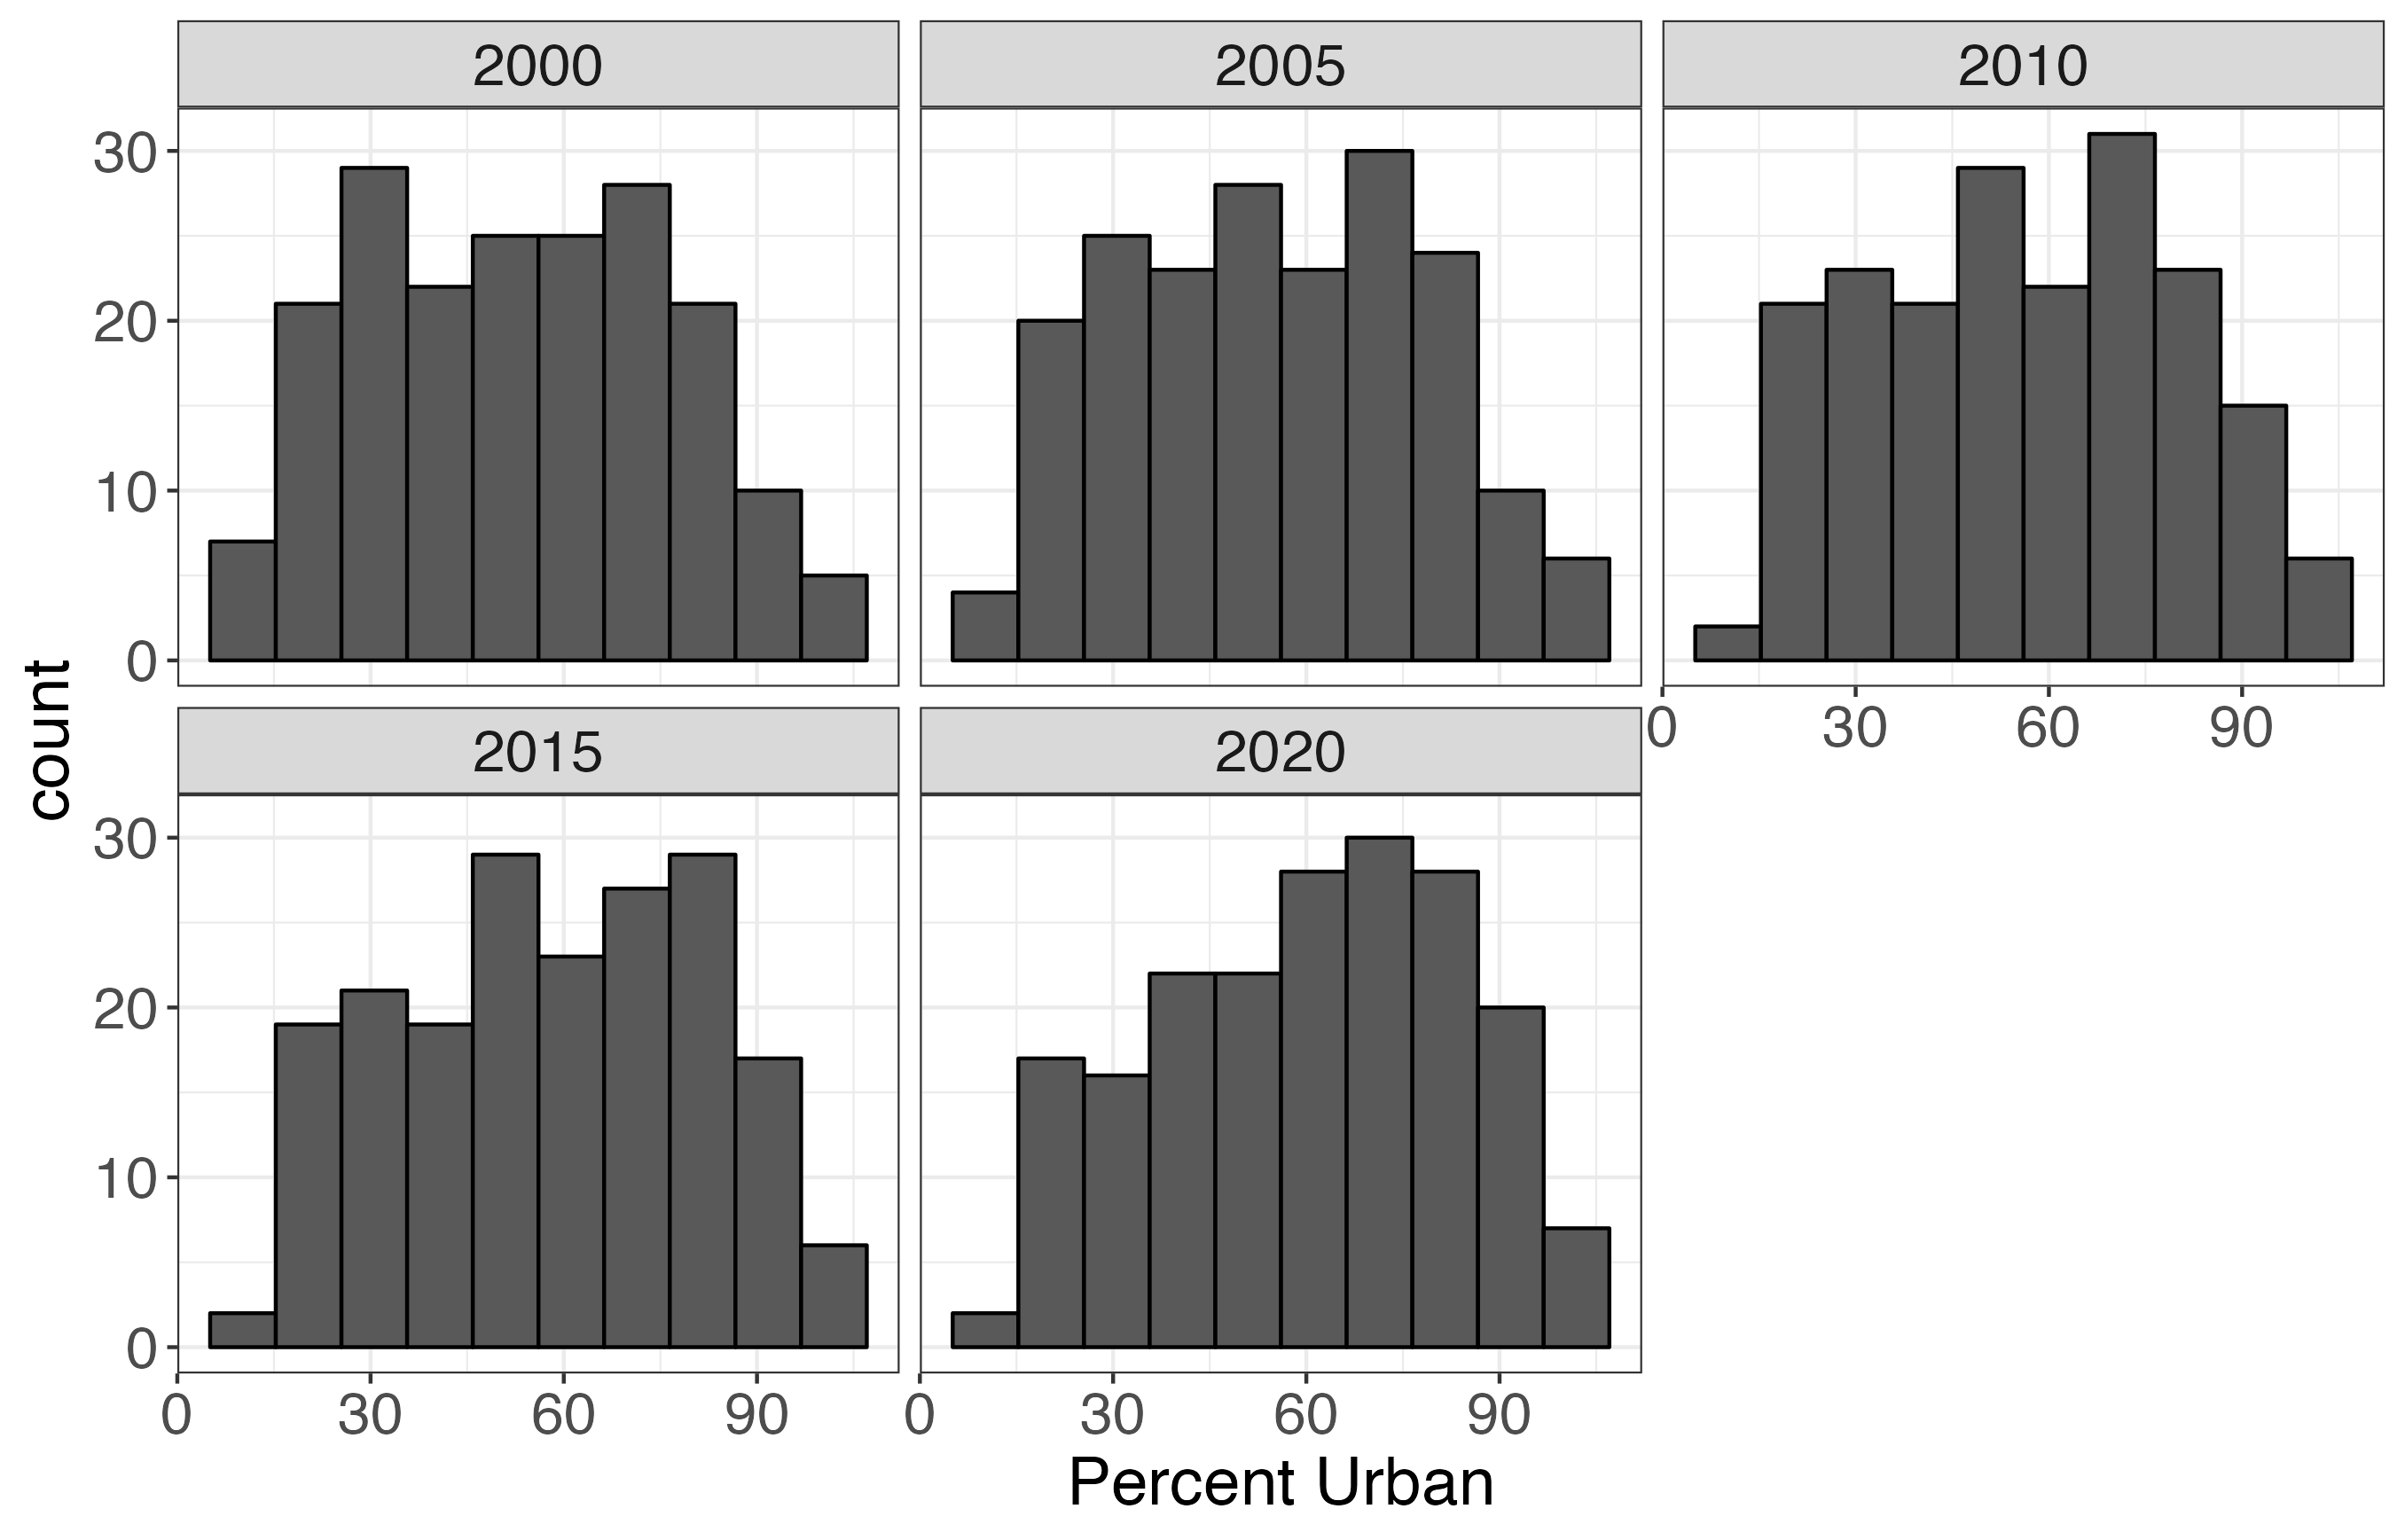
\includegraphics[scale=0.3]{urban_hist_years.png}

\end{frame}

\begin{frame}{Stratified Descriptive Statistics: Graphical}
We can also use side-by-side boxplots rather than side-by-side histograms. It may be easier to see the slightly increasing trend in mean percentage urban over year:

\vspace{0.3cm}

\centering 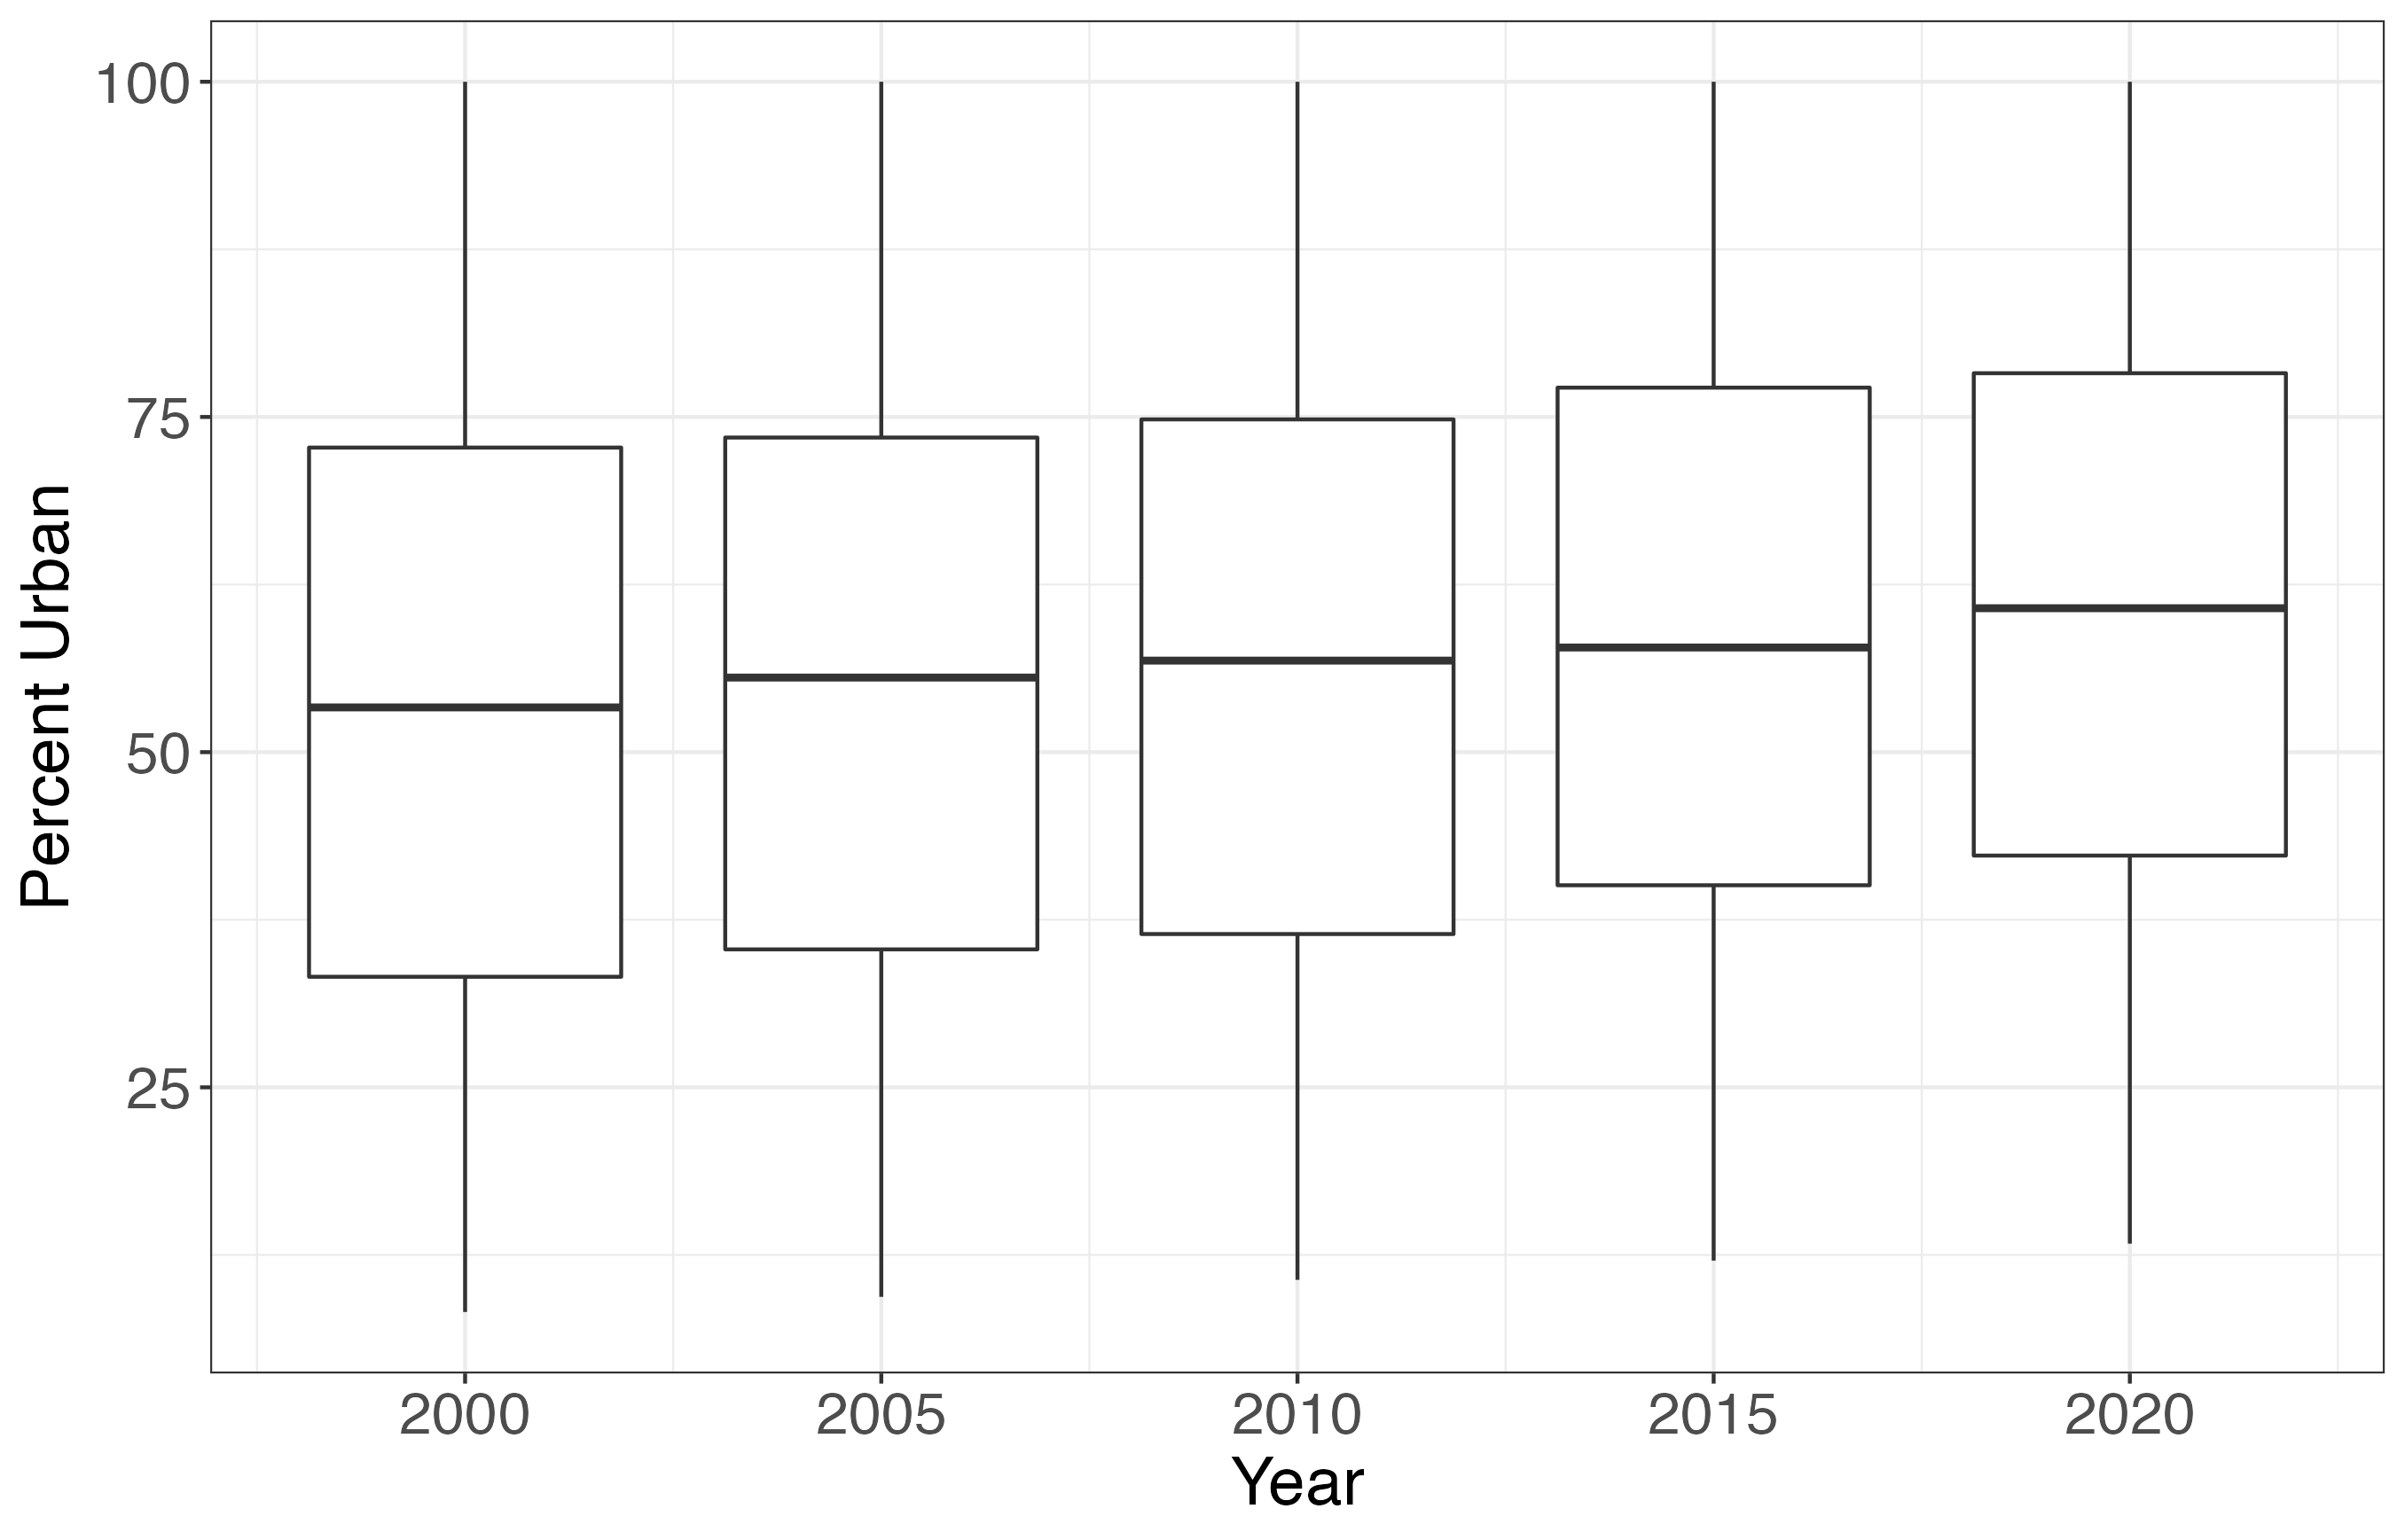
\includegraphics[scale=0.3]{urban_box_years.png}
\end{frame}

\begin{frame}{Stratified Descriptive Statistics: Graphical}
Scatters are a useful tool for summarizing the relationship between two quantitative variables. Below we plot median percent urban over all countries from years 2000 to 2020:

\vspace{0.3cm}

\centering 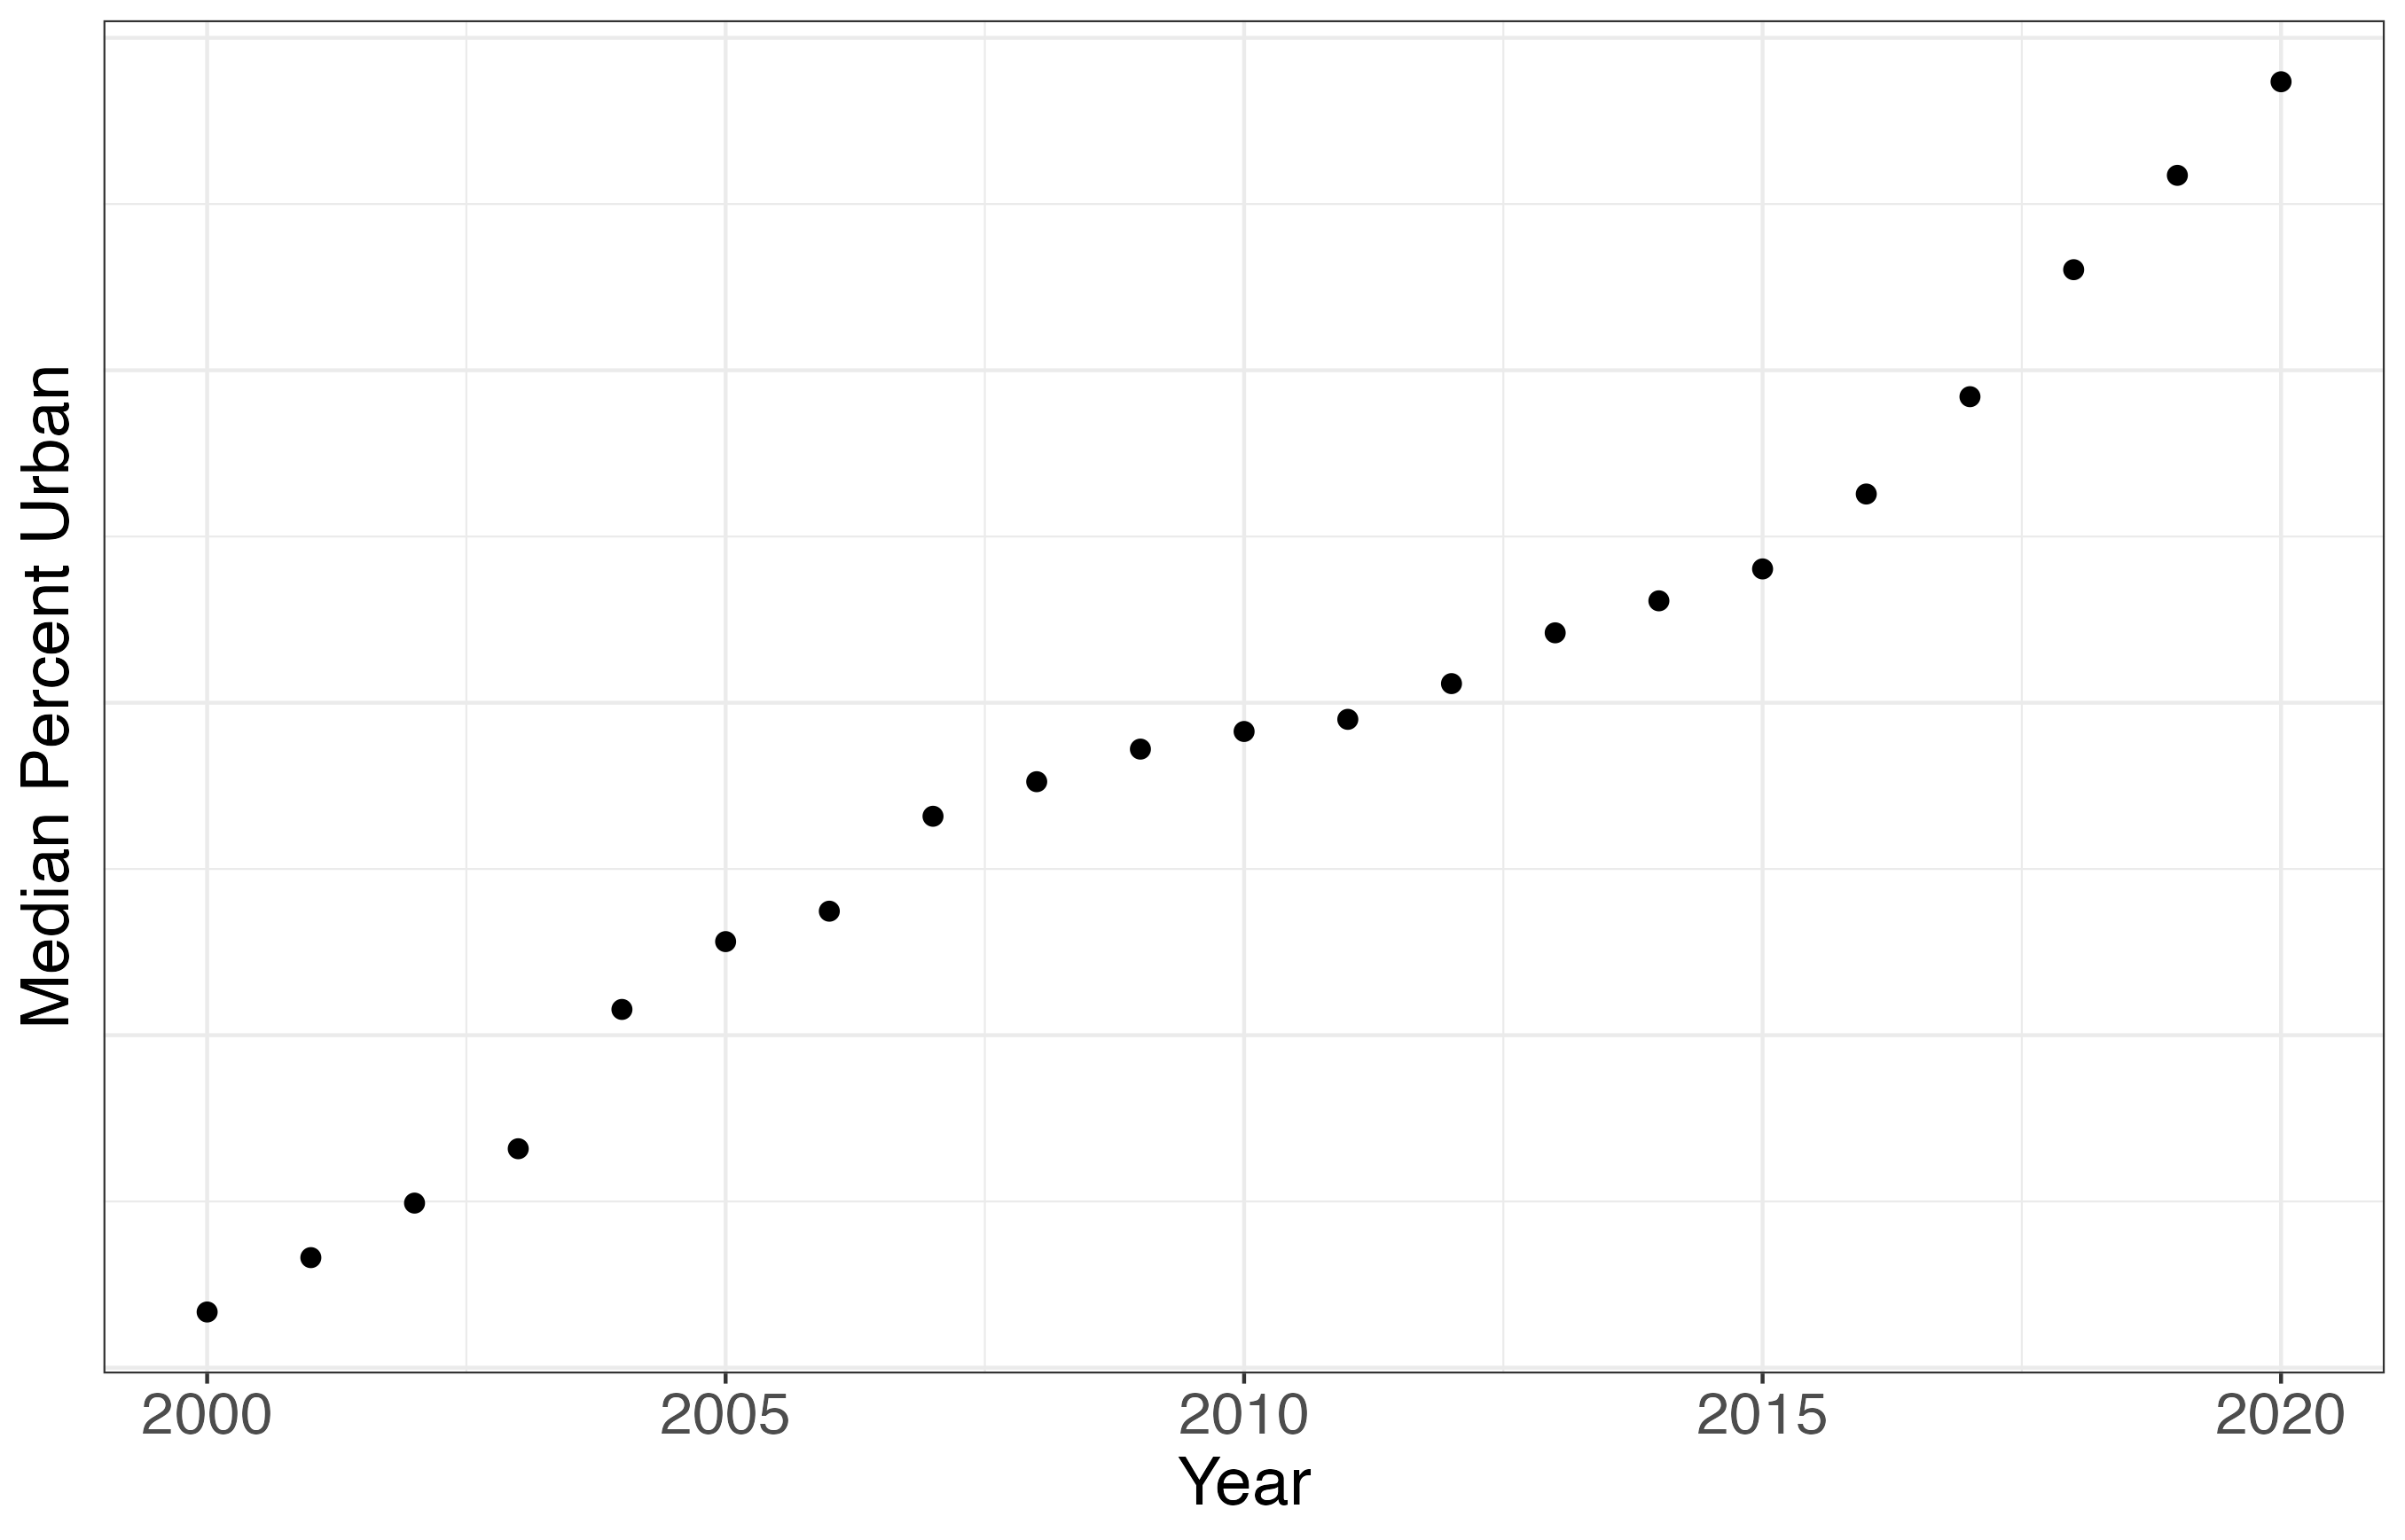
\includegraphics[scale=0.3]{urban_scatter.png}

\end{frame}

\begin{frame}{Descriptive Statistics in R}
This is just a small taste of the many possibilities when it comes to tools for summarizing data.

\vspace{0.3cm}

We’ll spend more time discussing descriptive statistics in Discussion Section, including how to generate numerical summaries and graphical summaries like these (or better ones!) in \texttt{R}.

\vspace{0.3cm}

You’ll also get practice on homework assignments and your data analysis project!

\end{frame}

\section{Statistical inference}

\begin{frame}{Descriptive statistics vs. Inferential statistics}
content...
\end{frame}

\begin{frame}{Motivating example}
Kelsey and Brian have quite a few slides on FEV... we should use something else here
\end{frame}

\begin{frame}{Precision vs. Accuracy}
Not sure why these slides are here. Is this the best fitting place for them?
\end{frame}

\subsection{Normal/t distributions}

\subsection{Central Limit Theorem}

\section*{References}
\begin{frame}
% to enforce entries in the table of contents
\end{frame}

\end{document}